\chapter{Software implementation}\label{cap.software}

In this chapter, we explain the algorithm that we have designed for solving the visual people tracking problem and its software implementation. 

\section{System overview}

The main contribution of this work is to develop a tracking algorithm that utilizes both a neural network and do not miss the real time operation. To do so we use the tracking-by-detection framework, and combine people detection using a neural network, somehow slow but very accurate, and link these detections with a regular feature tracking, very quick but prone to drift. 

The architecture of the system is summarized in the diagram \ref{software1}. Its inputs is a sequence of frames coming from a directory and its output is a CSV file. This file has the structure of the MOT's evaluation software requires. We divided the computing in two threads, the \textit{object detector thread} and the \textit{tracking thread}. The first is responsible of given a frame compute their pedestrian detections and send them to the \textit{tracking thread}, and the second one, it computes the tracking procedure frame to frame. In addition, when a new detection appears it combines with the tracker, this is called \textit{data association}, and finally it saves the results of the algorithm. We called data association to the process of combining a detection with the blobs. This is different to the data association concept in the tracking-by-detection nomenclature. In our algorithm the data association, like in the tracking-by-detection nomenclature, is the tracking module which links the detections with the blobs.



\begin{figure}[H]
\centering         
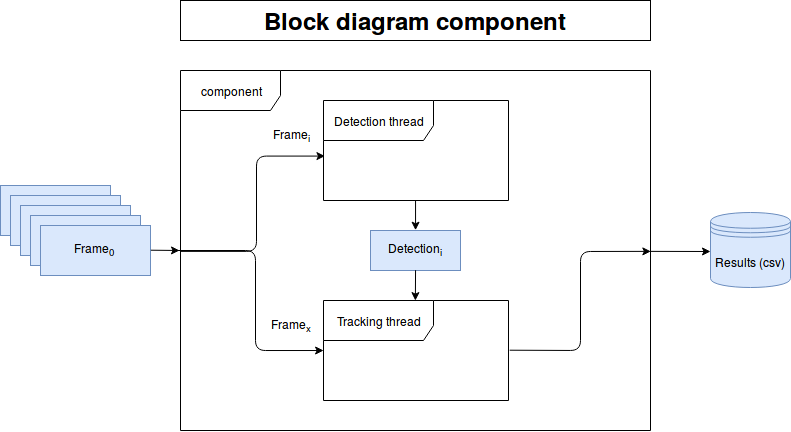
\includegraphics[width=12cm]{flows/bloque.png}
\caption{Block diagram of the component.} \label{software1}
\end{figure}


%Temporally the system works as follows. The algorithm starts, first of all it launches the \textit{object detector thread}, which begins to compute the detections of the first frame. Meanwhile, the \textit{tracking thread} remains idle, waiting for the detections. When the object detector finishes, it sends the initial detection to the tracking thread and at the same time starts to compute the detections on the next new frame. When the tracking thread receives a detection, it begins to compute the tracking between frames. Considering that the threads are not synchronized, the object detection thread goes ahead of the tracking thread, it will have a detection which the tracking thread could not incorporate, thus, it saves the detections in a shared buffer. When the tracking thread arrives to a frame that has got a detection it has a mechanism to mix detection with the blobs, this detection has been buffered, what it is called data association module, in addition it has a person re-identification module, to solve some possible identity incongruities, then it will continue computing the tracking.
%We can observe this temporal process in the next figure \ref{software2}, when $T$ represents a temporal step. When the object detector thread finishes computing all the detections it will \textit{die} and when the tracking thread process all the frame it dies too and the component it.


Temporally the system works as follows. When the algorithm starts, first of all it launches the \textit{object detector thread}, which begins to compute the detections of the first frame. Meanwhile, the \textit{tracking thread} remains idle, waiting for the detections. When the object detector finishes, it sends the initial detection to the \textit{tracking thread} and at the same time starts to compute the detections on the next new frame. When the \textit{tracking thread} receives a detection, it begins to compute the tracking between frames. Considering that the threads are not synchronized, the \textit{object detection} thread goes ahead of the \textit{tracking thread}, it will have a detection which the \textit{tracking thread} could not incorporate, thus, it saves the detections in a shared buffer. When the \textit{tracking thread} arrives to a frame that has got a detection it has a mechanism to mix detection with the blobs, this detection has been buffered previously, what it is called data association module, in addition it has a person re-identification module, to solve some possible identity incongruities, then it will continue computing the tracking.
We can observe this temporal process in the next figure \ref{software2timin}, when $T$ represents a temporal step. When the object detector thread finishes computing all the detections it will \textit{die} and when the tracking thread process all the frame it dies too and the component it. 


\begin{figure}[H]
\centering         
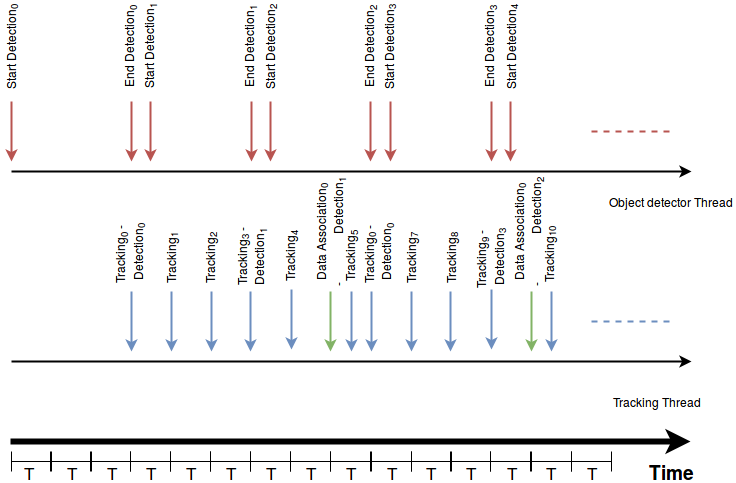
\includegraphics[width=14cm]{timesDiagram/timing3.png}
\caption{Timing of the component.} \label{software2timin}
\end{figure}


In the figure \ref{introTracking3} there is a flow chart of the algorithm. The object detector thread reads images, processes the forward pass of the neural network and saves the detections in the shared buffer, it repeats this sequence until it has processed all the predefined list of frames. In another hand, the main tread activates the object detector thread and waits till it gets the first detection, after this, it starts the tracking algorithm. It reads the images and computes the motion of all the regions of interest. However, at beginning of each cycle it checks whether it has got newer detection coming from the \textit{object detector thread} to mix it in.

\begin{figure}[H]
	
\centering

\subfigure[Tracking thread.]{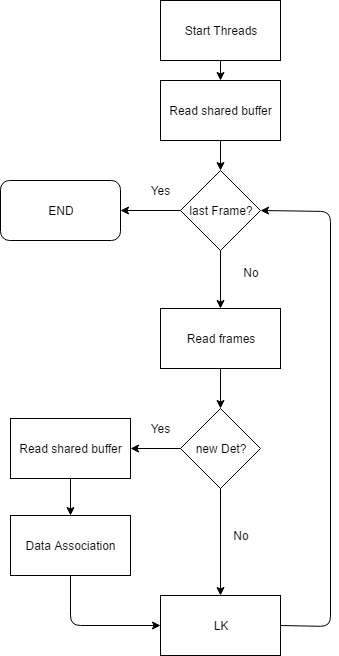
\includegraphics[width=5cm]{flows/arc.png}}
\subfigure[Object detector thread.]{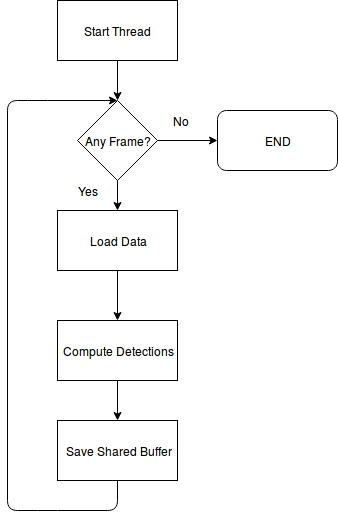
\includegraphics[width=5cm]{flows/detetc.png}}\\


\caption{Flow chart of the system.}
\label{introTracking3}
\end{figure}

We represent each person with a bounding box, in this bounding box \ref{systemintro2} we extract some features and compute how they move through the frames, based on the movement of those features we will infer the movement of the bounding box, therefore, the movement of the person.


\begin{figure}[H]
		
\centering

\subfigure[Detection.]{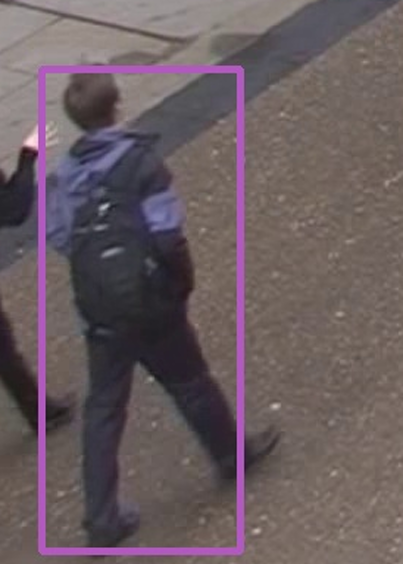
\includegraphics[width=3cm]{BoundingBox3/bounding1.png}}
\subfigure[Points.]{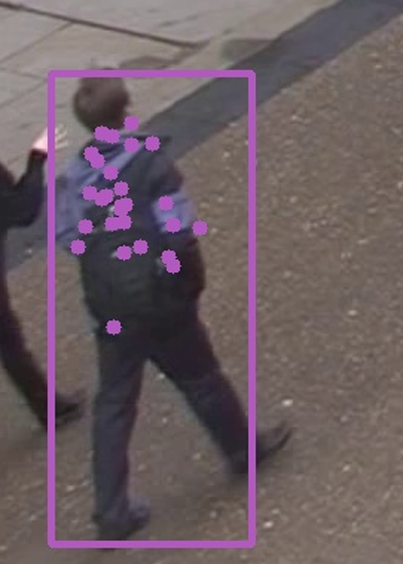
\includegraphics[width=3cm]{BoundingBox3/ppints1.png}}
\subfigure[Displacement.]{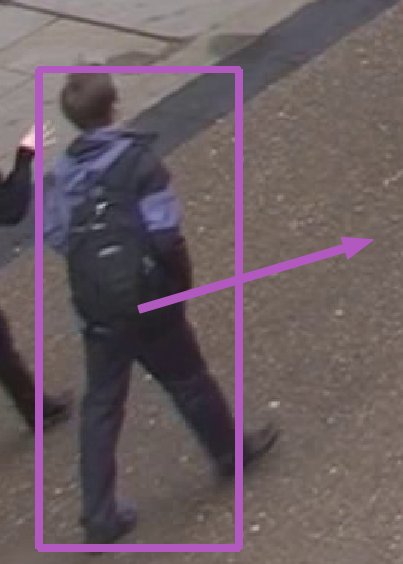
\includegraphics[width=3cm]{BoundingBox3/arrow1.png}}\\
\caption{Image and motion vectors of a moving camera sequence.}
\label{systemintro2}
\end{figure}




With this approach we accomplish to join two different technologies, we can exploit their benefits and reduce their drawbacks. We can get an accurate detection every $30$ frames and in between, we link those detections with the feature-based tracking module. In this way, we reduce the fragility of the tracking, it tends to miss feature points and cause a drift of the estimation, with a new detection, that corrects that drift. In addition, we compensate the slowness of the detection with the speed of the feature tracking.



Next we explain each part in detail.

\section{Object detector thread}



As we stated previously we compute the pedestrian detector based on a CNN. This types of systems are very accurate but slow. We are constraint by execution time of the chosen detector, it takes $0.92$ seconds for compute each detection, this allows us to get a new detection after $30$ frames. The \textit{object detector thread} reads images from the directory, processes the forward pass of the neural network and saves the detections in the shared buffer, it repeats this sequence until it has processed all the predefined list of frames. This process is summarized in \ref{objectThresPseudo}.


\begin{algorithm}
%\caption{Object detection thread}\label{euclid}
\begin{algorithmic}[1]
\State \textbf{Input:} sequencesOfImages
\State \textbf{Output:} sharedVariable
\State $fpsRate = 30$
\State $numberFramesSequences = size(sequencesOfImages)$
\State $network = network.init()$
\State $listIndex = createList(FPS,numFramesSequences)$
\Procedure{Run}{}
\For {$indexImage$ in $listIndex$}
\State $image = read(indexImage)$
\State $detection = network.forward(image)$
\State $sharedVariable = detection$
\EndFor
\EndProcedure
\end{algorithmic}
\caption{Object detection thread}\label{objectThresPseudo}
\end{algorithm}

We selected the Single shot multibox detector (SSD) as object detector, because it has got the best balance between performance and speed, in section \ref{valdiation:det} we make a comparison of the available detectors. This detector was trained with the union of the COCO and the VOC07 dataset and implemented on TensorFlow. Finally, in \ref{objectDetector1} we can observe the result of this step.


\begin{figure}[H]
\centering         
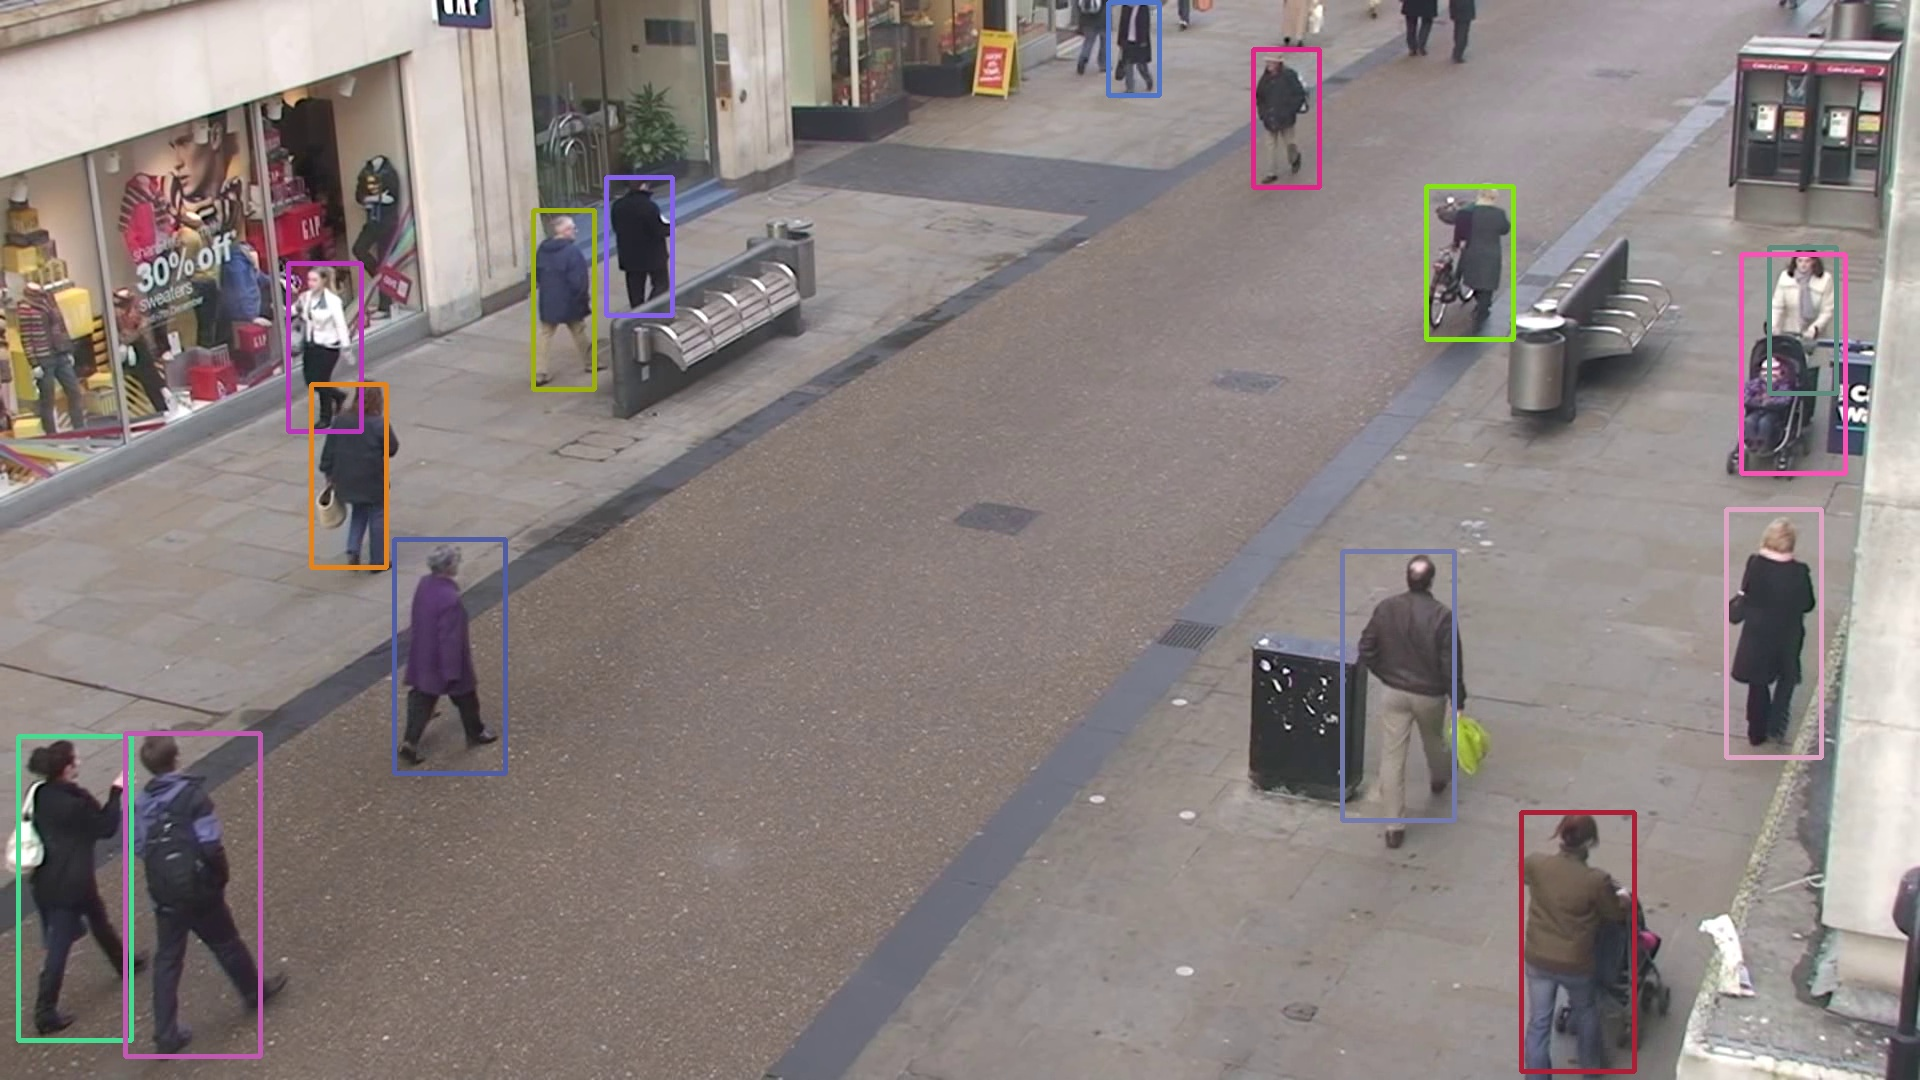
\includegraphics[width=12cm]{intro/deteccions.jpg}
\caption{Detections of the algorithm.} \label{objectDetector1}
\end{figure}


\section{Tracking thread}




The essence of the \textit{tracking thread} it is the tracking module, called LK in the figure \ref{introTracking3}. It stands for Lucas-Kanade algorithm, due it is the method that we used in this work. This module for each detection computes its displacement by computing the displacement of the features inside this bounding box. 



\subsection{Feature extraction}

It computes for each blob at each step. For extracting the features, we use the OpenCV routine \texttt{goodFeaturesToTrack()}, this function determines strong corners on an image, according the Shi-Tomasi method. His parameters and values are the following:
 
\begin{itemize}

\item \texttt{image}, input image

\item \texttt{maxCorners}, maximum number of corners to return. If there are more corners than are found, the strongest of them is returned. We set this value experimentally to 60.
\item \texttt{qualityLevel}, parameter characterizing the minimal accepted quality of image corners. We set this value experimentally to 0.1.
\item \texttt{minDistance}, minimum possible Euclidean distance between the returned corners. We set this value experimentally to 2.
\item \texttt{mask}, optional region of interest. Not used.
\item \texttt{blockSize}, Size of an average block for computing a derivative covariation matrix over each pixel neighborhood. We set this value experimentally to 7.
\item \texttt{useHarrisDetector},  Parameter indicating whether to use a Harris detector. Not used.
\item \texttt{k},  Free parameter of the Harris detector. Not used.

\end{itemize}

We applied an equalization transformation to the image before the feature extraction, to obtain more high contrast points, in \ref{exper:validation} we perform a comparision of several preprocessing techniques. We can observe the results of this process in the figure \ref{solution2} and for all the blobs it looks like \ref{solution3}.


\begin{figure}[H]
\centering         
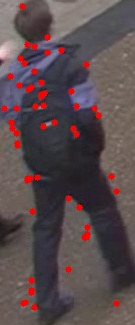
\includegraphics[width=3cm]{implementation/pointsEQU.jpg}
\caption{Shi-Tomasi points on a person.} \label{solution2}
\end{figure}

%
%\begin{algorithm}
%\caption{Object detection thread}\label{euclid}
%\begin{algorithmic}[1]
%\Procedure{Detection}{}
%%\State $A tracker prodcues a trajectory by tracking the point forward in time$
%%\State $network \gets \textit{patlen}$
%\State $network = network.init()$
%\State $FPS = 30$
%\State $FRAMES SEQUENCES = num of files(sequences)$
%\State $LIST_INDEXs = createList(FPS,FRAMES_SEQUENCES)$
%\For {(each object $LIST_INDEX$)}
%\State $image = read()$
%\State $detection = network.forward(image)$
%\State $sharedVariable = detection$
%\EndFor
%\EndProcedure
%\end{algorithmic}
%\end{algorithm}


\begin{figure}[H]
\centering         
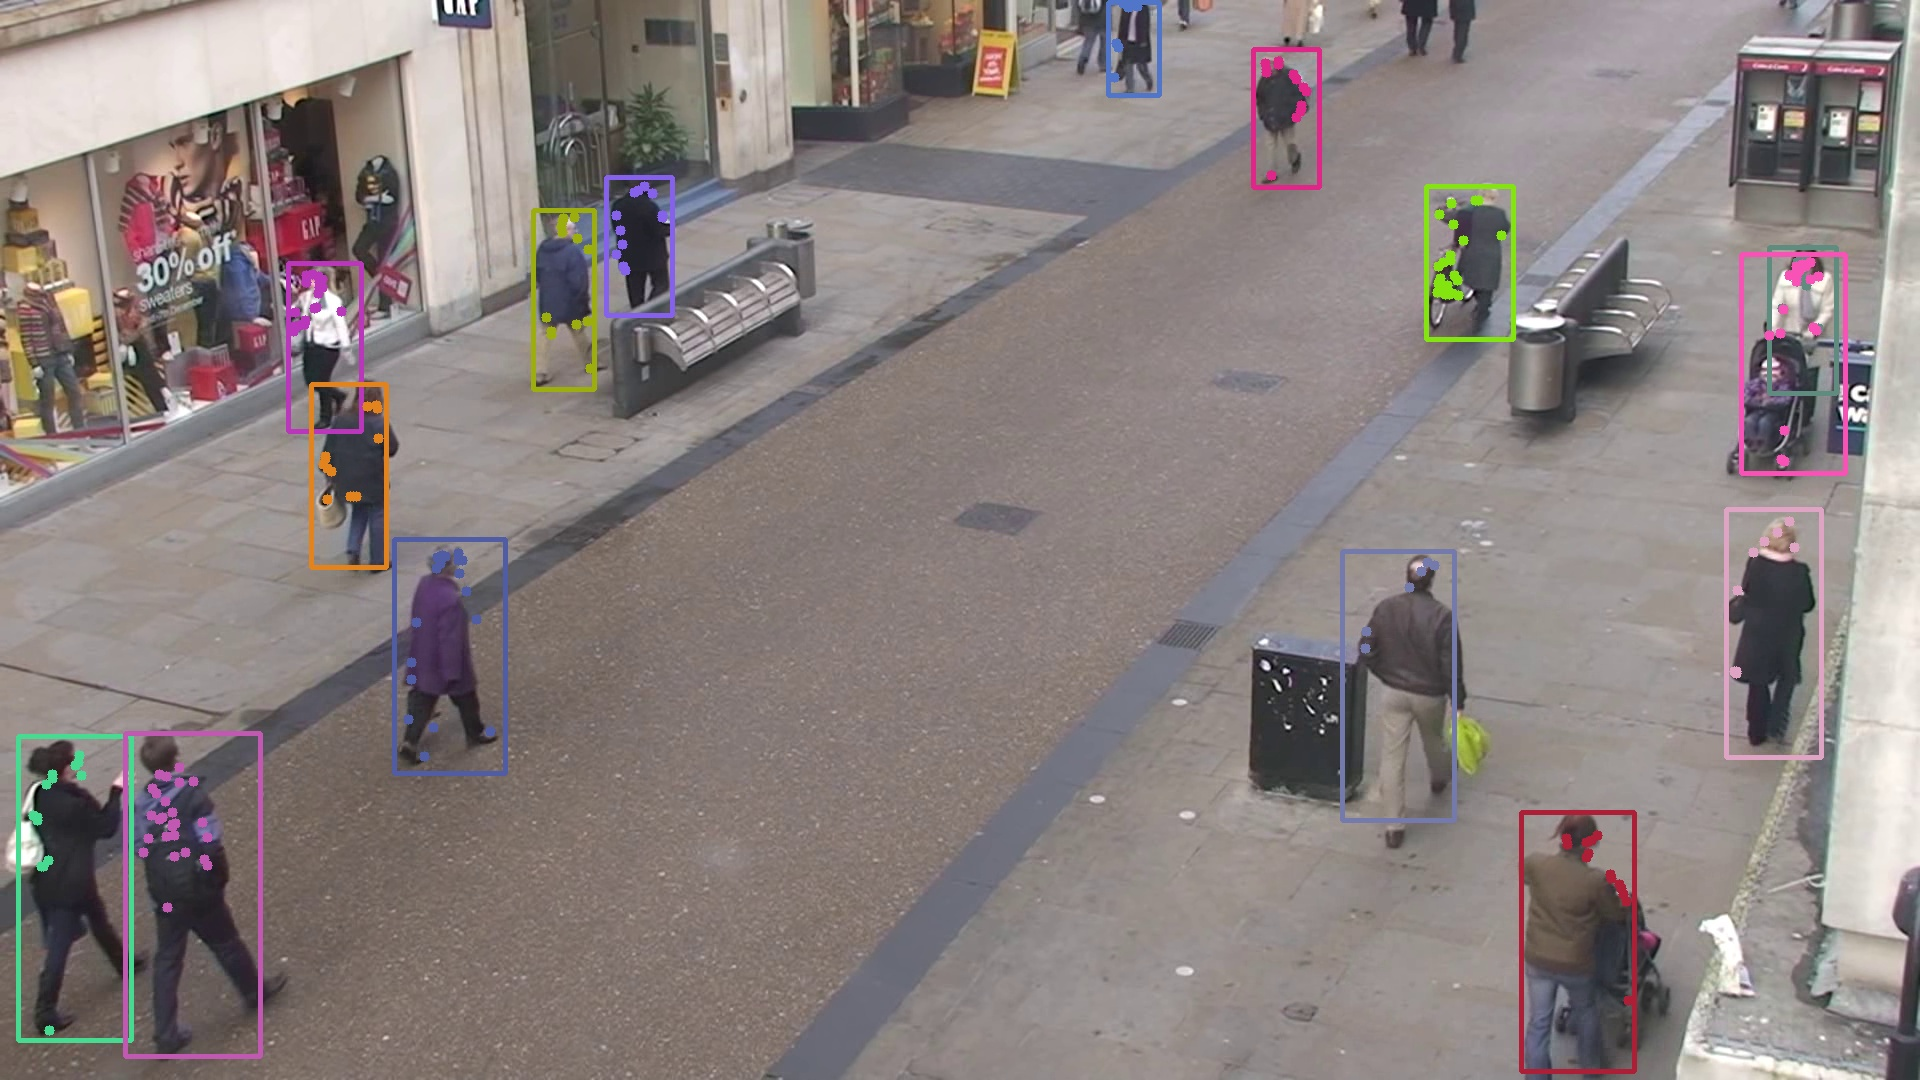
\includegraphics[width=10cm]{intro/pounts.jpg}
\caption{Blobs with their feature points.} \label{solution3}
\end{figure}

 
%\begin{algorithm}
%\caption{Forward-backward method}\label{euclid}
%\begin{algorithmic}[1]
%\Procedure{FB}{}
%\State $A tracker prodcues a trajectory by tracking the point forward in time$
%\State $i \gets \textit{patlen}$
%%\BState \emph{top}:
%\If {$i > \textit{stringlen}$} \Return false
%\EndIf
%\State $j \gets \textit{patlen}$
%%\BState \emph{loop}:
%\If {$\textit{string}(i) = \textit{path}(j)$}
%\State $j \gets j-1$.
%\State $i \gets i-1$.
%\State \textbf{goto} \emph{loop}.
%\State \textbf{close};
%\EndIf
%\State $i \gets i+\max(\textit{delta}_1(\textit{string}(i)),\textit{delta}_2(j))$.
%\State \textbf{goto} \emph{top}.
%\EndProcedure
%\end{algorithmic}
%\end{algorithm}

\subsection{Feature matching}


Once we have all the detections with their feature points, we can compute its displacement, to do so,  we used the OpenCV's routine \texttt{calcOpticalFlowPyrLK()}, this function implements a sparse iterative version of the Lucas-Kanade optical flow with pyramids. And his parameters and values are the following:
 
\begin{itemize}

\item \texttt{prevImg}, first image.
\item \texttt{nextImg}, second image.
\item \texttt{prevPts}, vector of 2D points for which the flow needs to be found. 
\item \texttt{nextPts}, output vector of 2D points containing the calculated new positions of input features in the second image. 
\item \texttt{status}, output status vector, it tells you whether the flow has been found.  
\item \texttt{err}, each element of the vector is set to an error for the corresponding feature.
\item \texttt{winSize}, size of the search window at each pyramid level. We set this value experimentally to 15.
\item \texttt{maxLevel}, number of pyramid levels. We set this value experimentally to 4. 
\item \texttt{criteria}, parameter, specifying the termination criteria of the iterative search algorithm. We set this value experimentally to 10 iterations.
\end{itemize}



For the example's person we can observe the matching between the points of consecutive frames in figure \ref{solution4}.

\begin{figure}[hptb]
\centering         
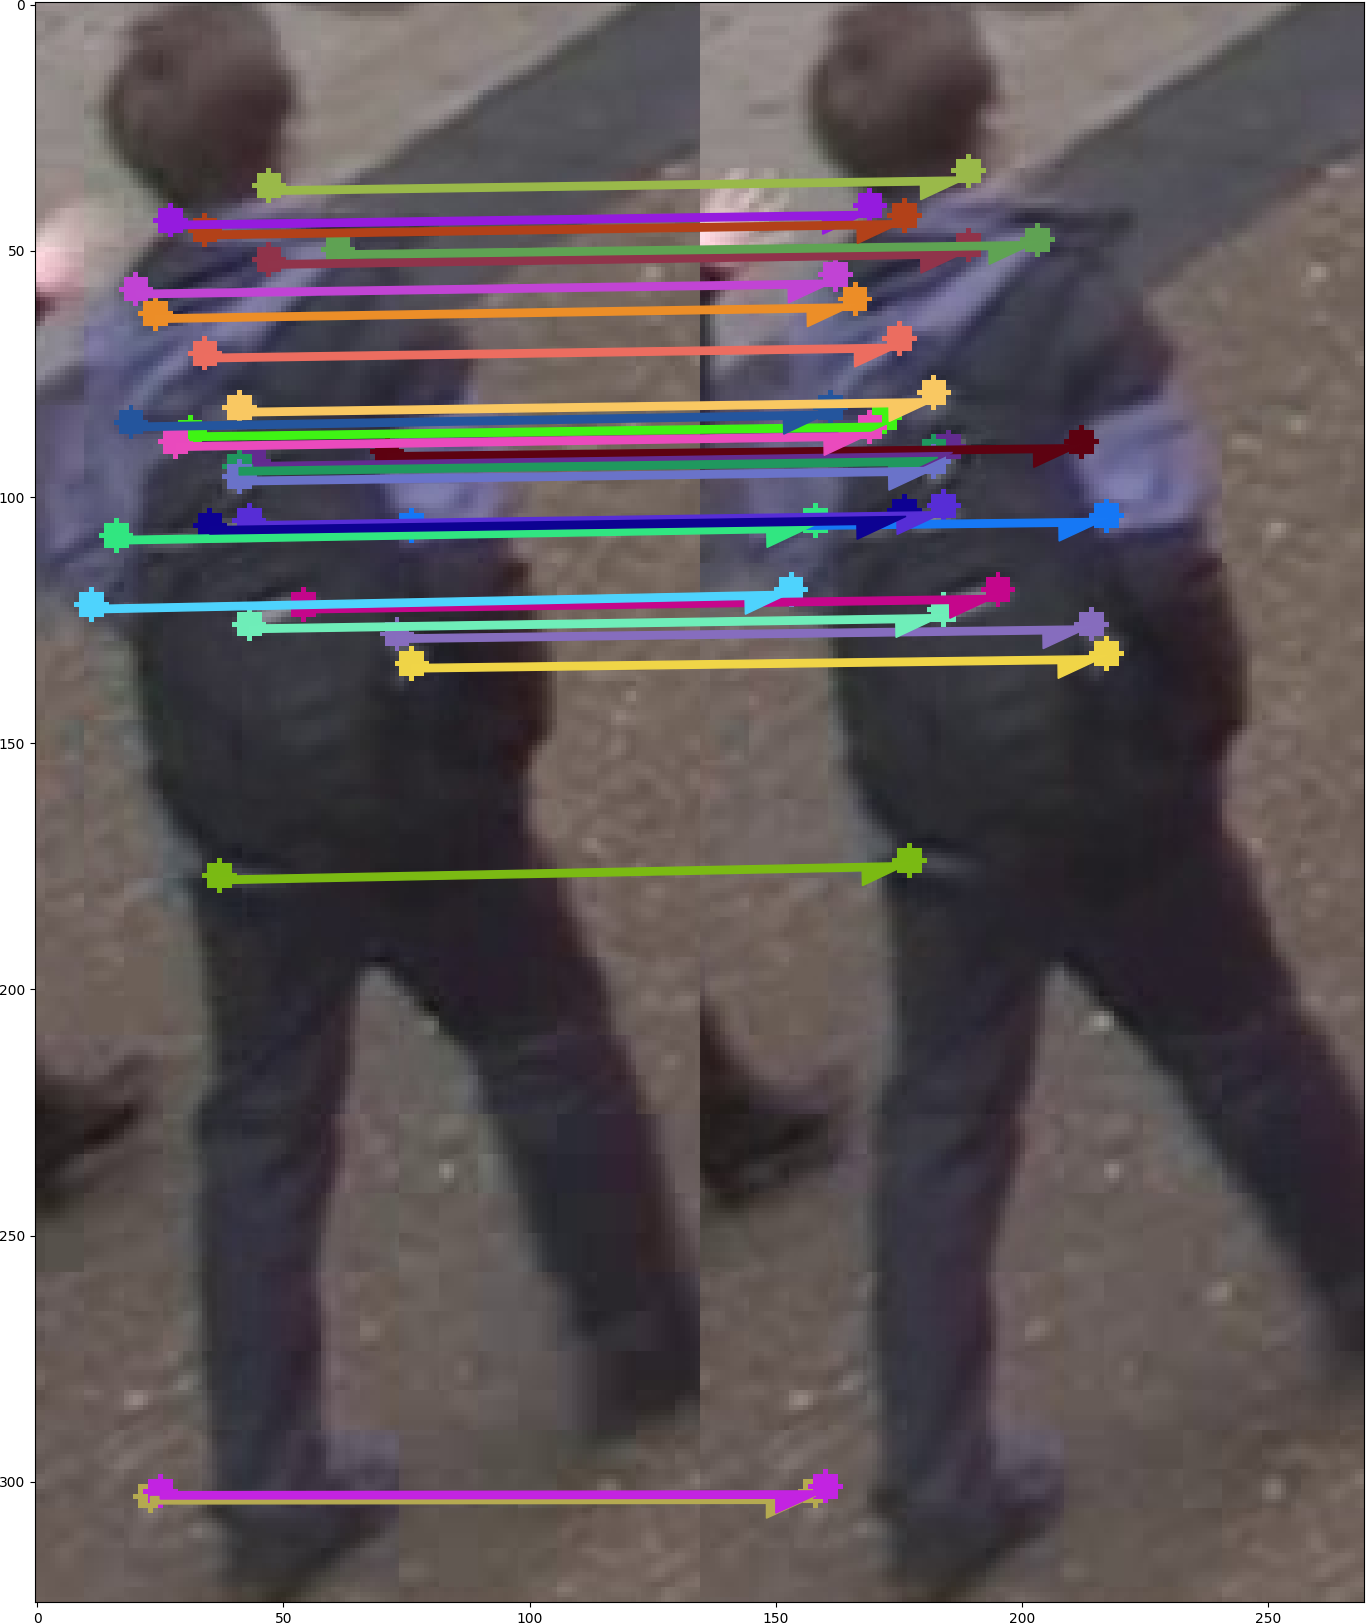
\includegraphics[width=0.3\linewidth]{implementation/matching.png}
\caption{Matched feature points.} \label{solution4}
\end{figure}




%--------------------------------

After this step we have a bunch of motion vectors, but some vectors in the bounding box do not belong to the pedestrian, and if we do not erase it will contribute to the motion computation. Usually this points belong to the static elements of the scene, like the floor or urban furniture, this points in terms of motion between subsequent frames will be very low or almost static. We can observe this fact plotting the displacement of this points and drawing it in the image, we can observe it at \ref{motion2}. So, we erase the points with a displacement smaller than a threshold. We set this value experimentally to 1.0. 

\begin{figure}[H]
		
\centering

\subfigure[Image points.]{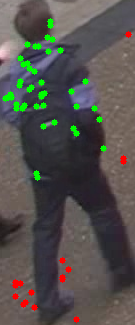
\includegraphics[width=2.5cm]{implementation/reejctMore.png}}
\subfigure[Displacement graphics.]{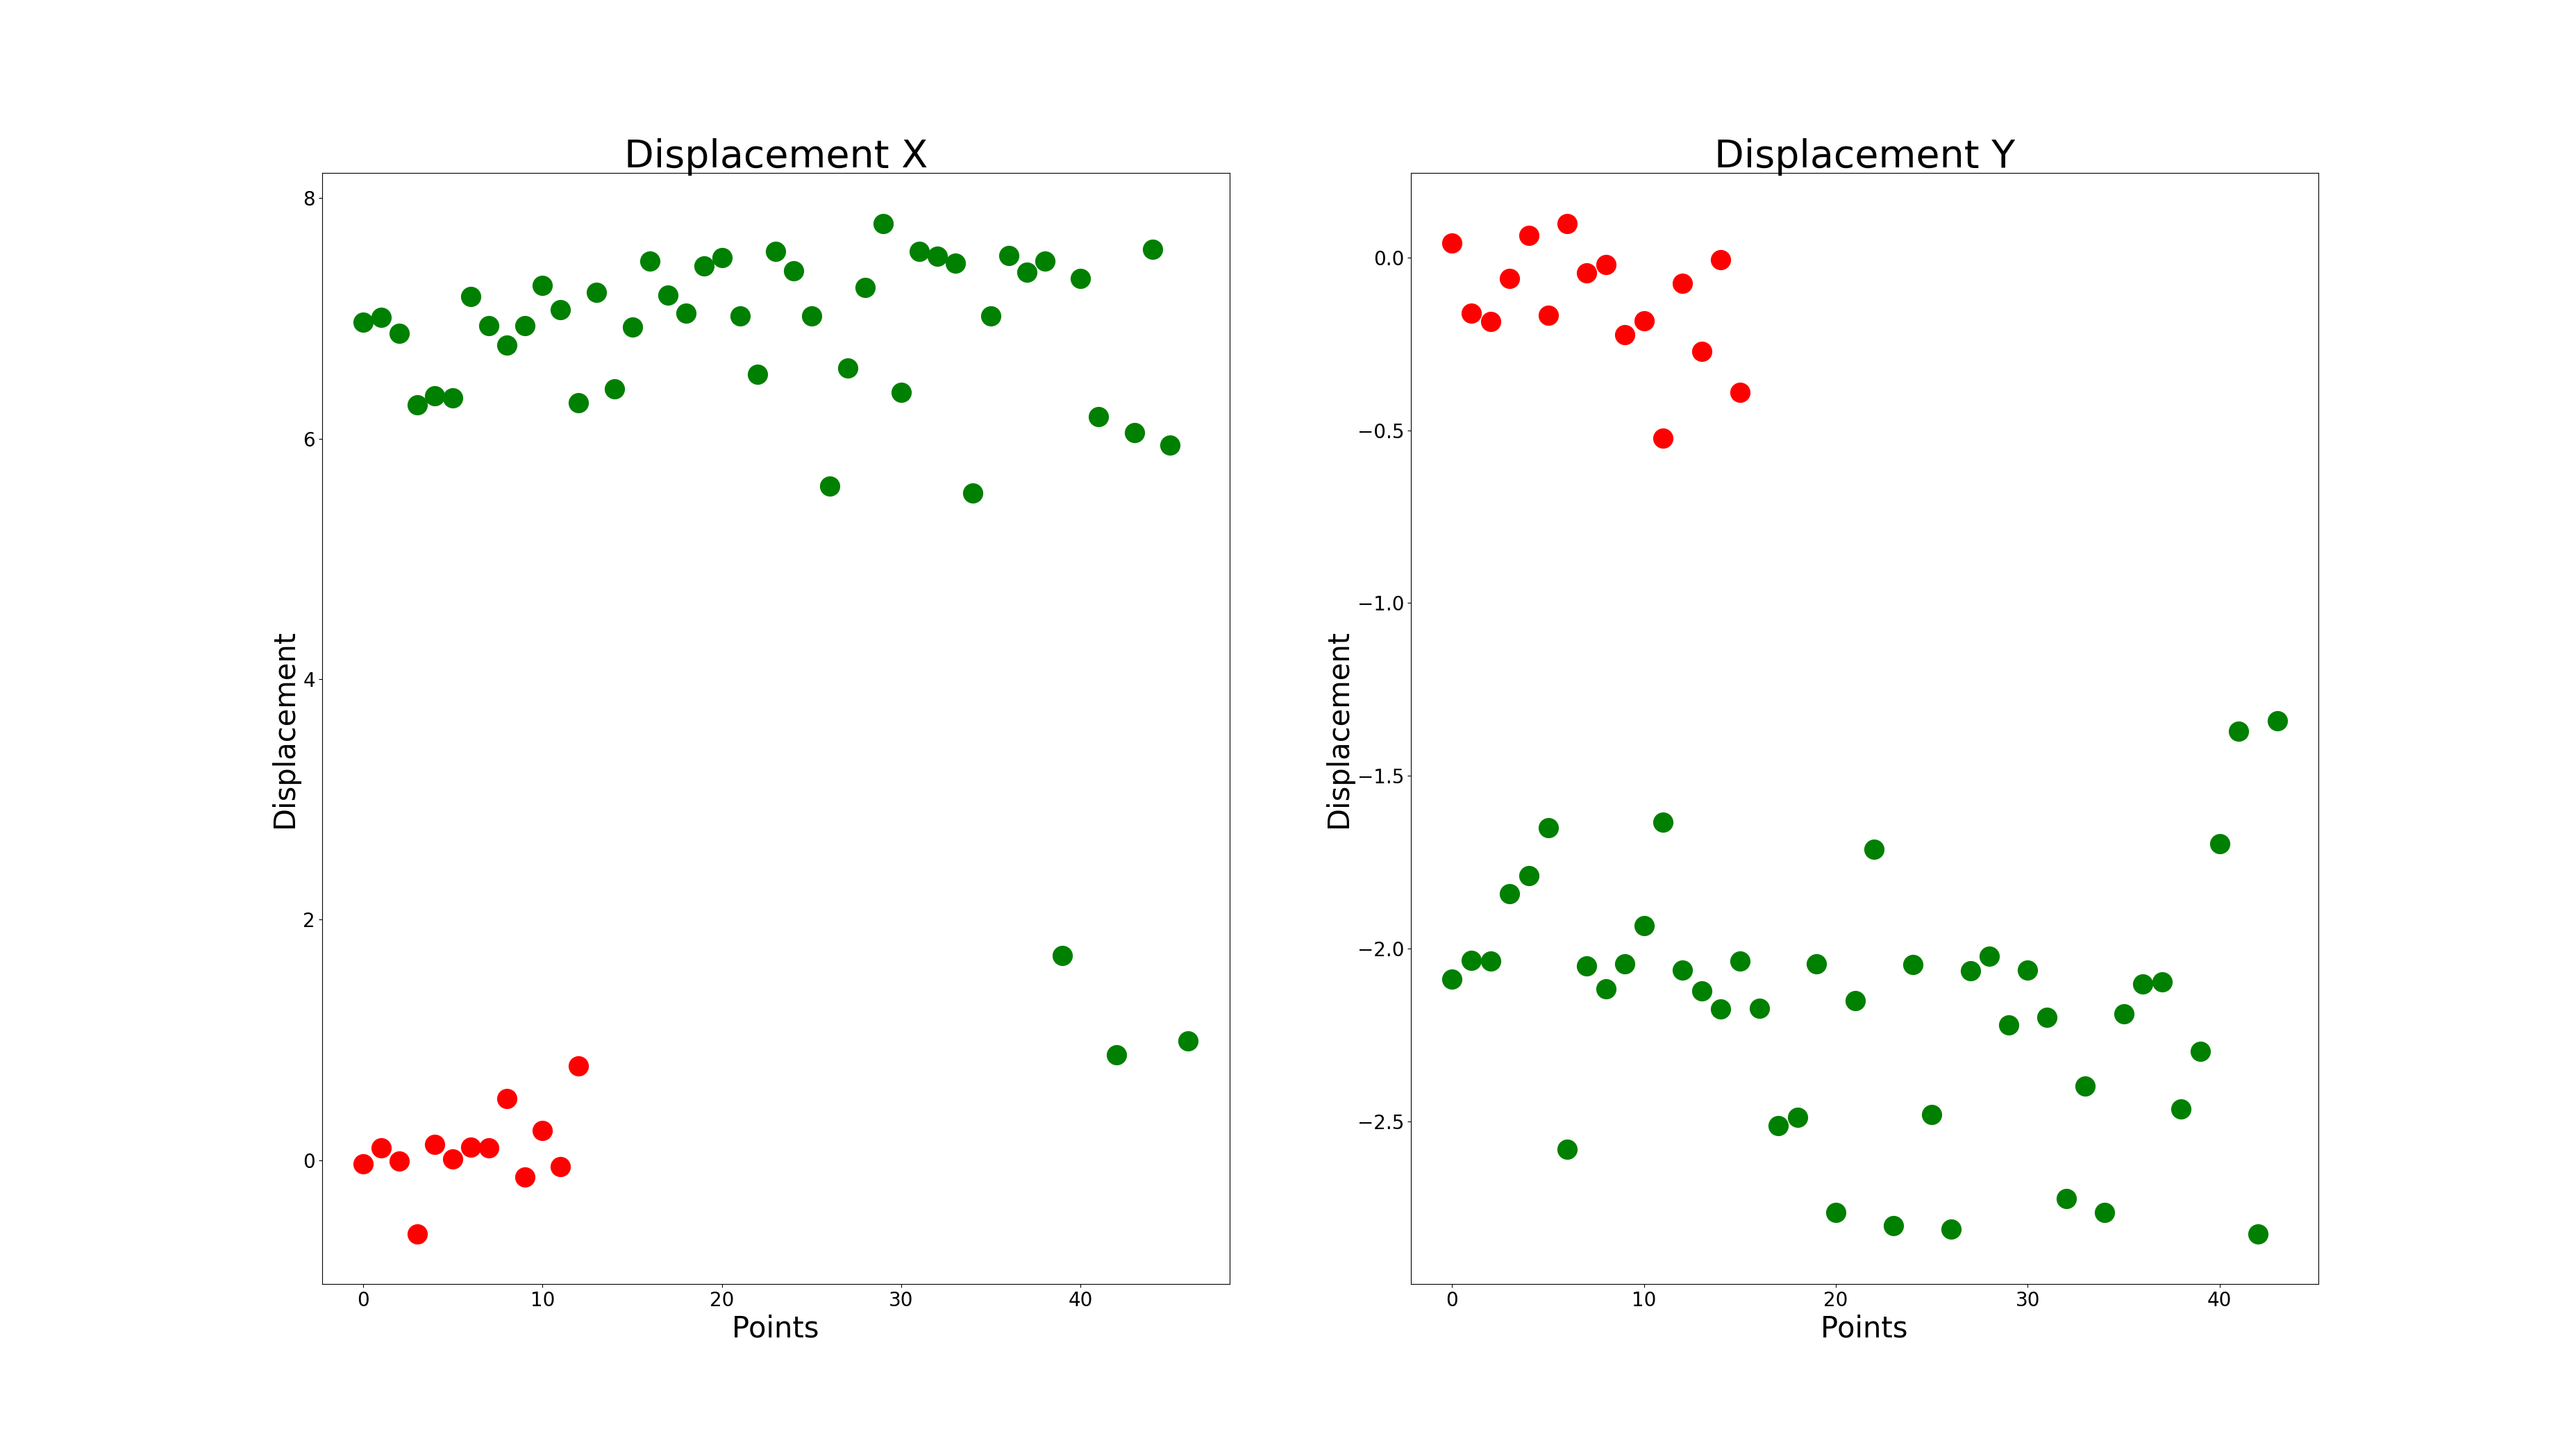
\includegraphics[width=13cm]{implementation/filterVeloPoints.png}}\\
\caption{Image and motion vectors.}
\label{motion2}
\end{figure}

But, this behavior will only work on sequences where the camera is fixed, in sequences produced by a moving camera it will not work, we can observe the plot of displacement vectors on a sequence acquired by a moving camera in \ref{motion3}. 

\begin{figure}[H]
		
\centering

\subfigure[Image points.]{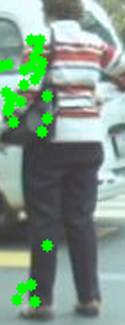
\includegraphics[width=2.5cm]{implementation/foto004.png}}
\subfigure[Displacement graphics.]{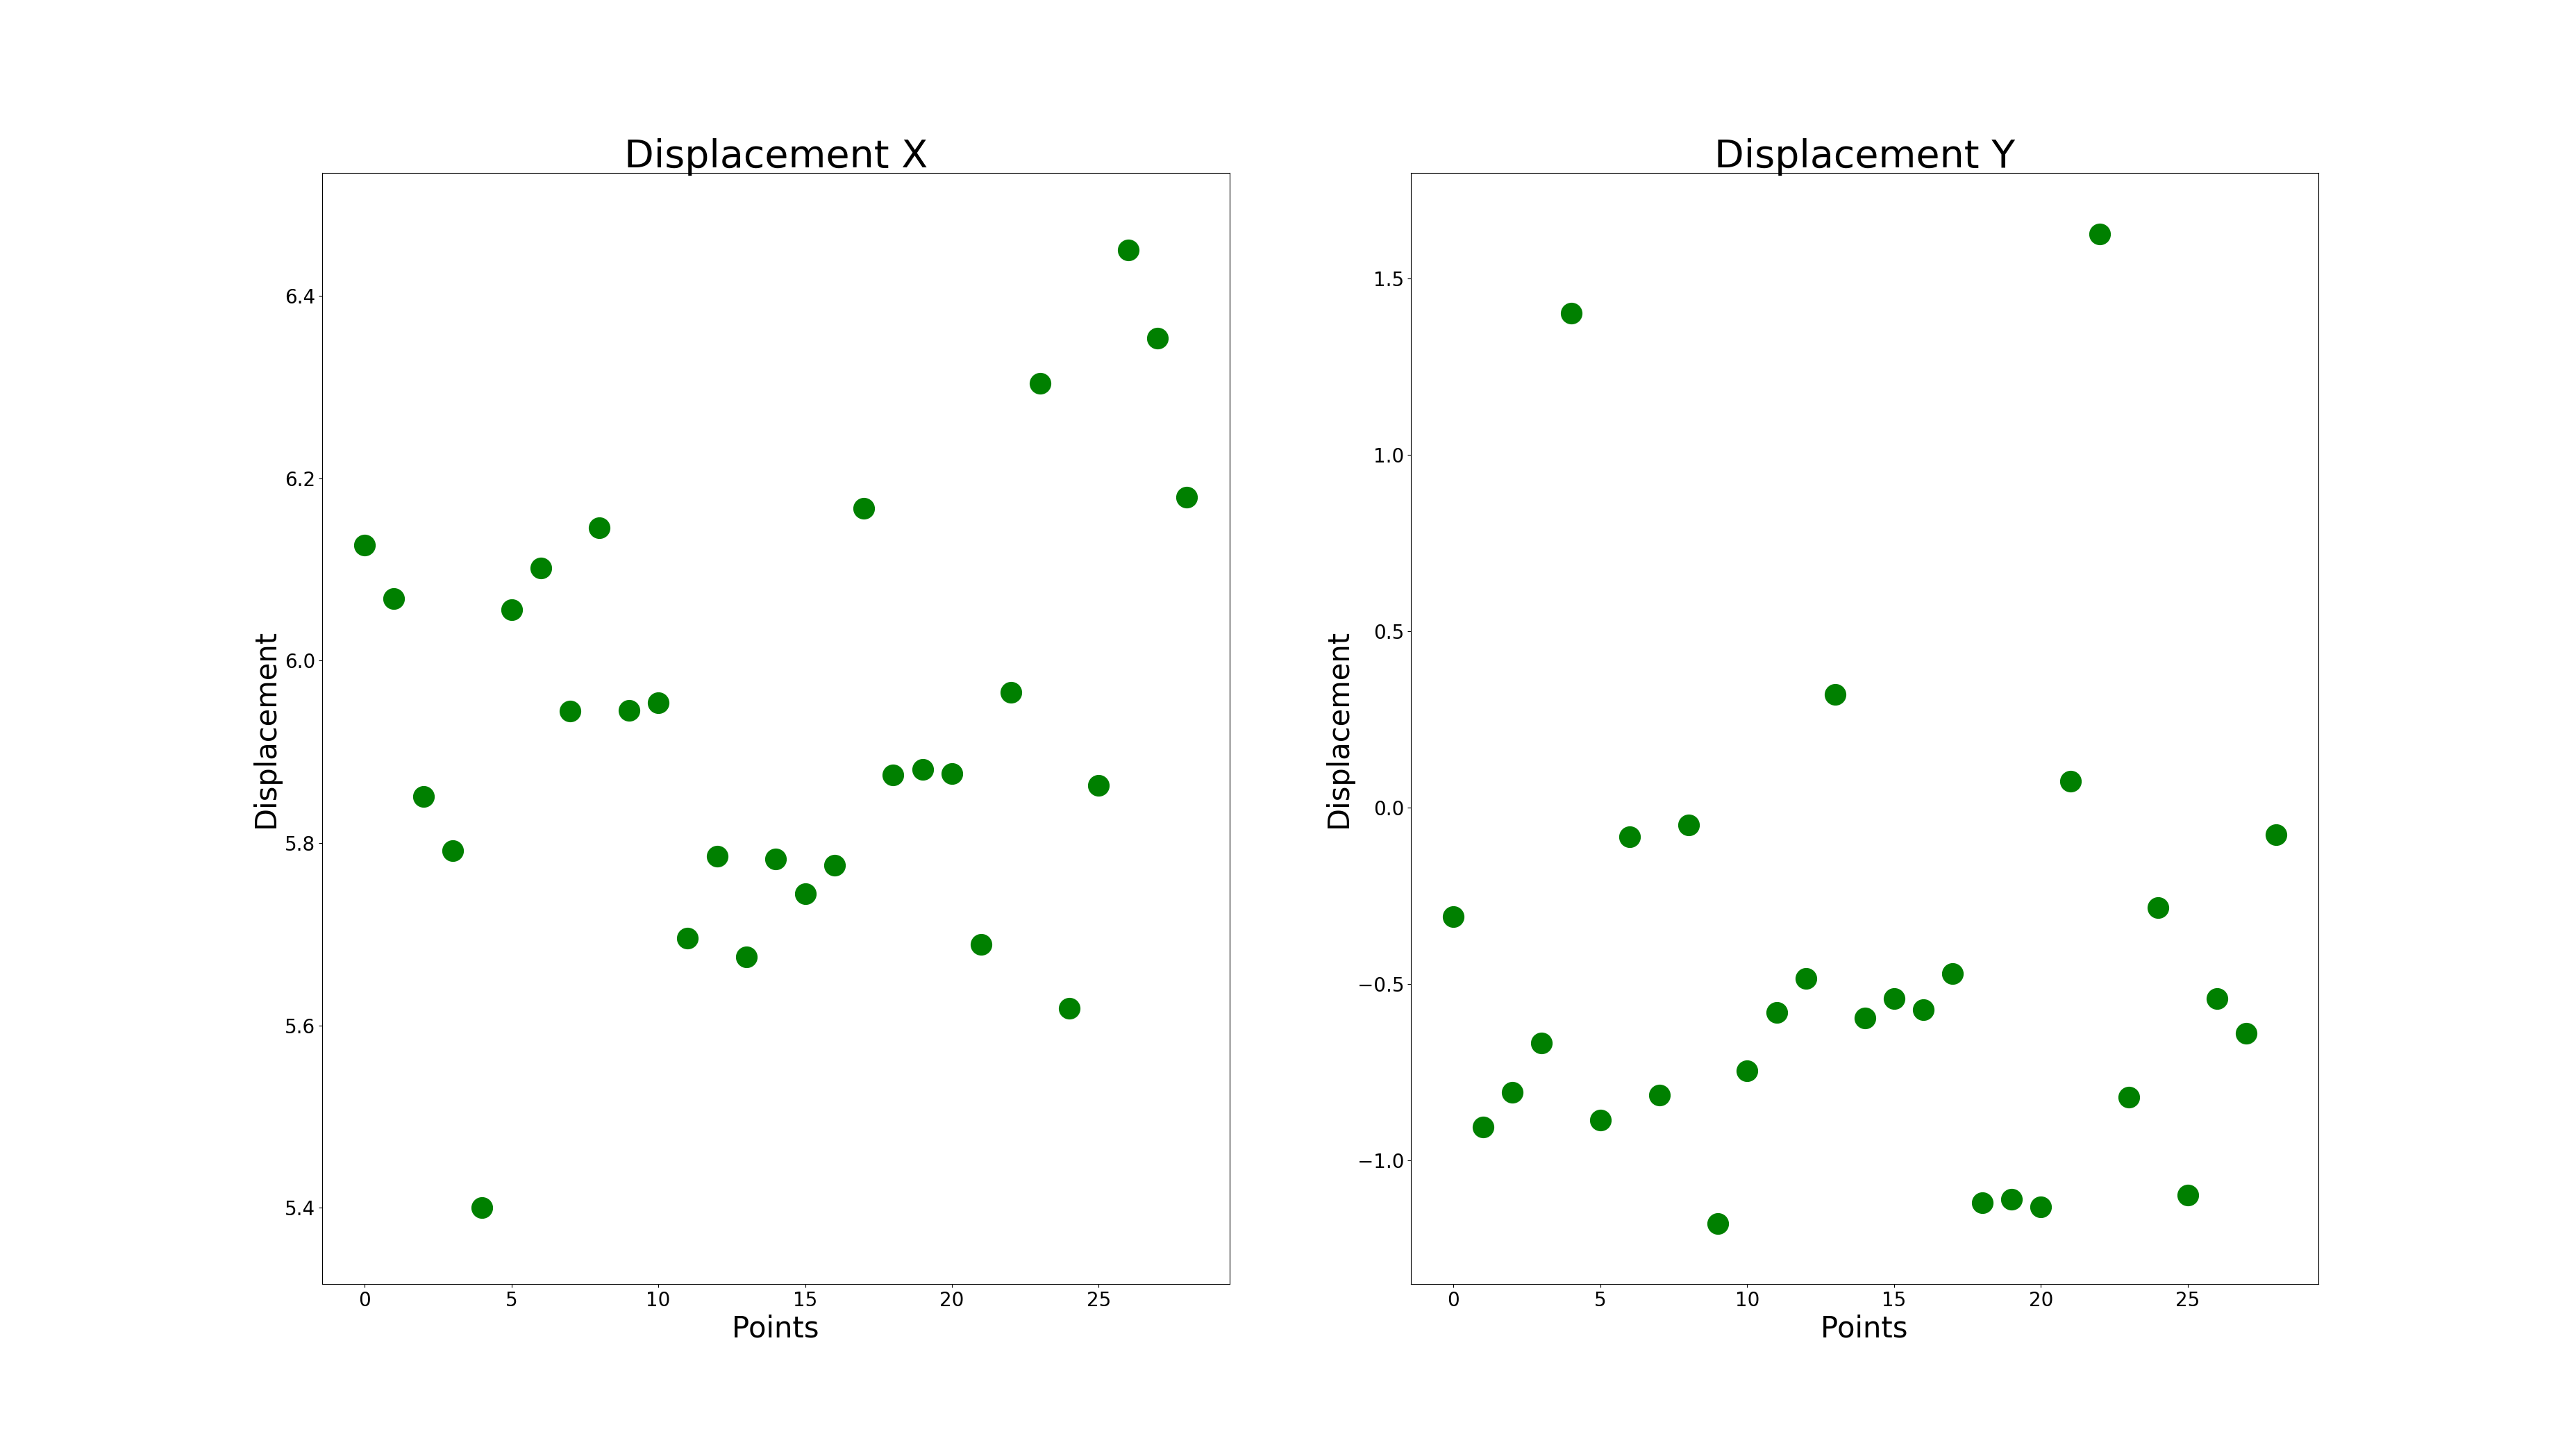
\includegraphics[width=13cm]{implementation/figurePoints.png}}\\
\caption{Image and motion vectors of a moving camera sequence.}
\label{motion3}
\end{figure}


\subsection{Blob matching}


Once we have the correct correspondaces, we compute the displacement as the median of all of them in each dimension. We also compute the change of the scale of the blob, it is computed as follows: for each pair of points, a ratio between current point distance and previous point distance is computed, bounding box scale change is defined as the median over these ratios. In the figure \ref{solution5} we can observe a representation of this displacement for each blob.


\begin{figure}[H]
\centering         
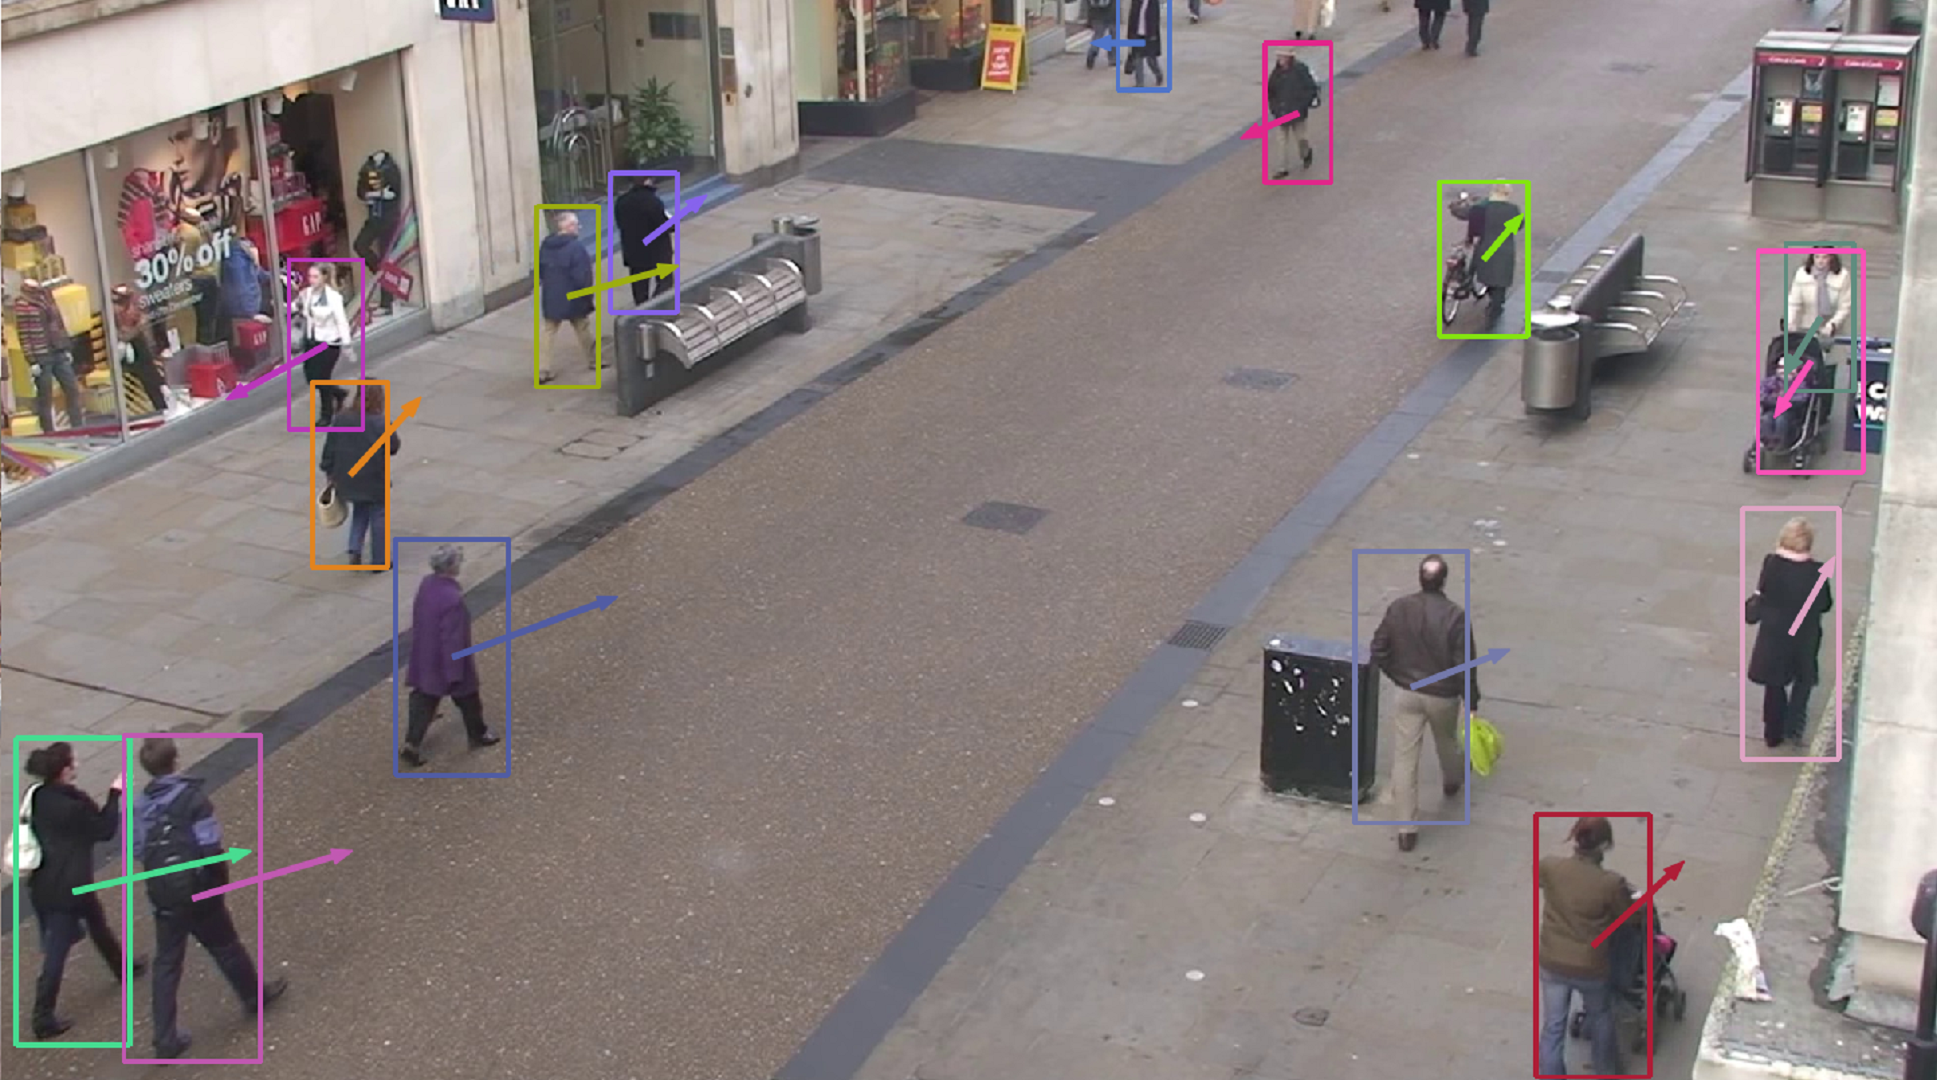
\includegraphics[width=10cm]{intro/alcover2.png}
\caption{Displacement of each blob.} \label{solution5}
\end{figure}


With this discplacement and the change in scale we can update the position of the blob in the next frame. In the figure \ref{solution4} we can observe the previous estimation and the new one. At this point we have solved the data association problem in the tracking-by-detection nomenclature.


\begin{figure}[H]
\centering         
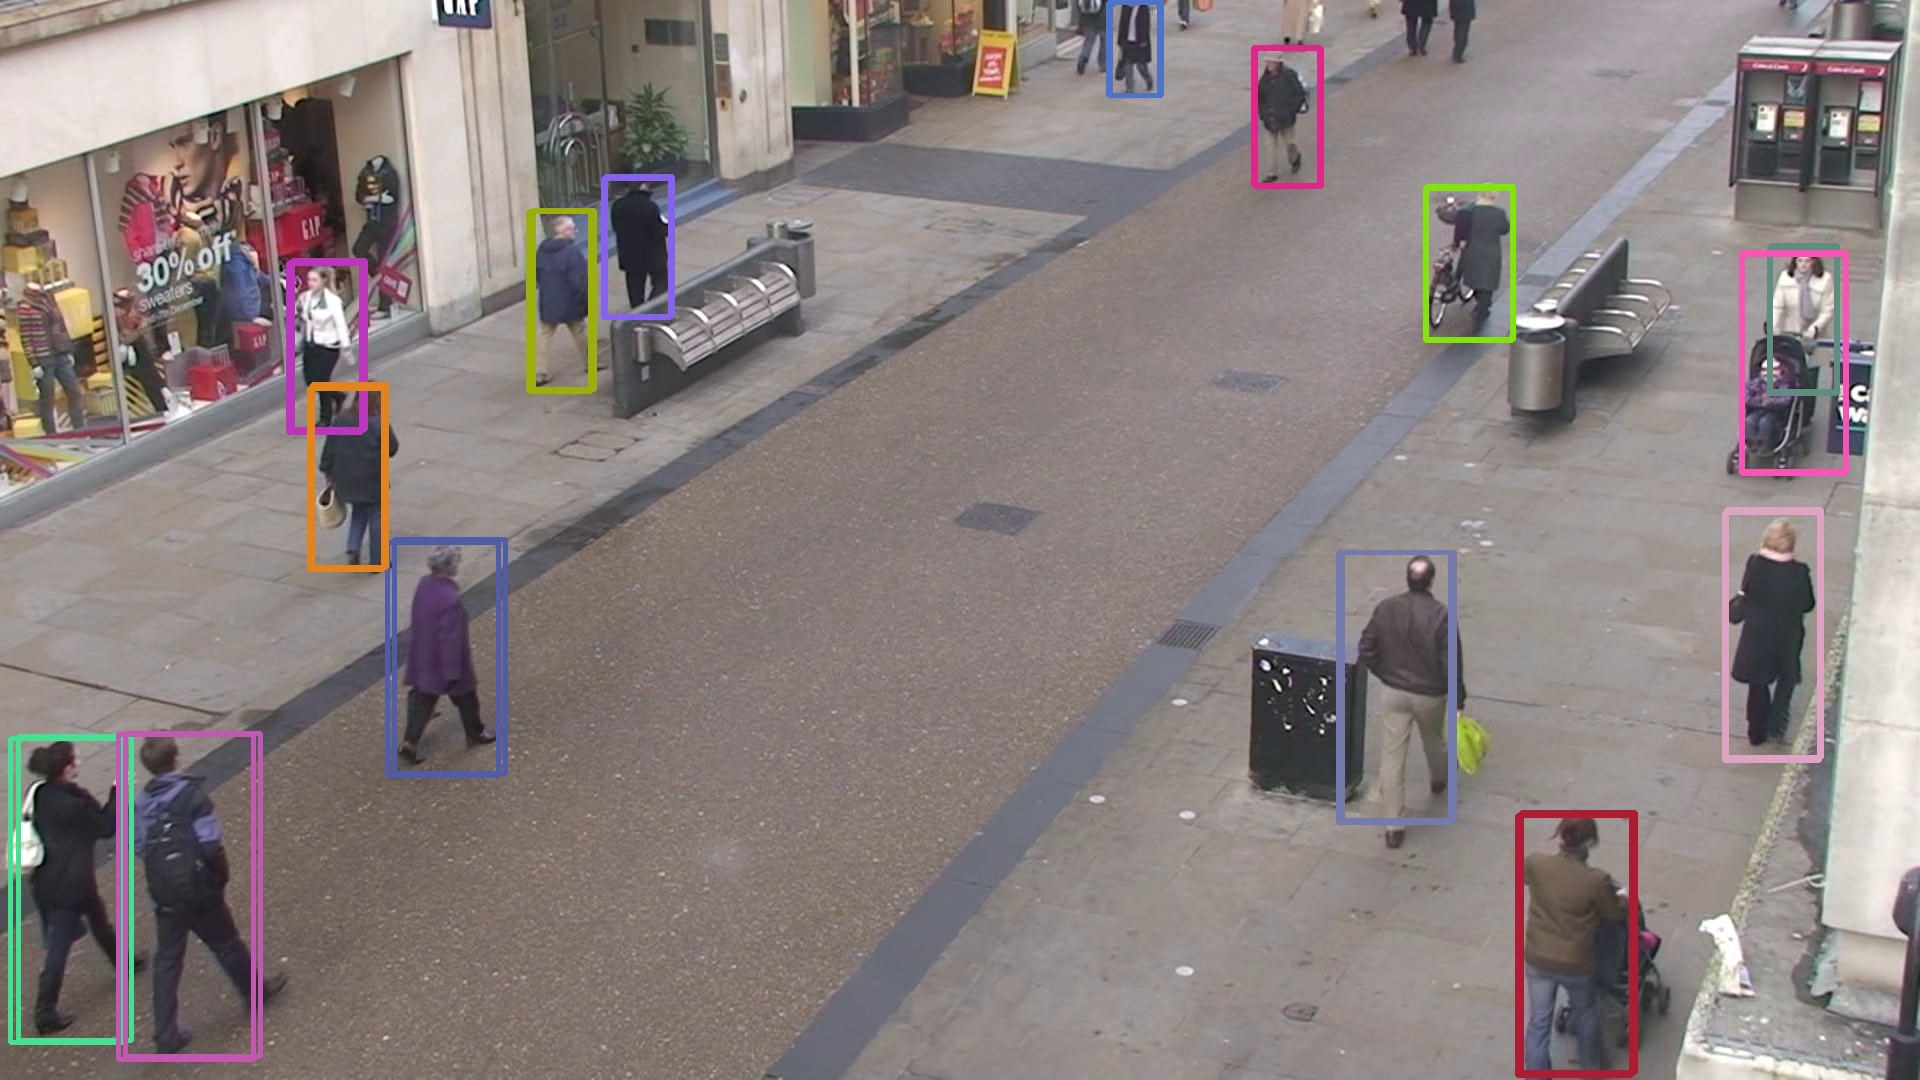
\includegraphics[width=10cm]{intro/deteccionsBLOB.jpg}
\caption{Uploaded estimation.} \label{solution4}
\end{figure}

%--------------

%In \ref{trackingModule} there is a pseudocode that summarizes these steps, this pseudocode given two temporal blobs, \textit{Blob1} and \textit{Blob2} computes its displacement in each coordinate and its change in scale. At this point, we have an implementation of the tracking algorithm given a set of bounding boxes.

In \ref{trackingModule} there is a pseudocode that summarizes these steps, this pseudocode given the current blob computes the new estimation, \textit{Blob1} and \textit{Blob2}, respectively. At this point, we have an implementation of the tracking algorithm given a set of bounding boxes.



\begin{algorithm}
%\caption{Object detection thread}\label{euclid}
\begin{algorithmic}[1]
\State \textbf{Input:} Blob1,Blob2 
\State \textbf{Output:} displacementX,displacementY,diffScale
%\Procedure{RUN}{}
\State $blob1Equ = equalize(Blob1)$
\State $features1 = cv2.goodFeaturesToTrack(blob1Equ)$
\State $blob2Equ = equalize(Blob2)$
\State $features2 = cv2.calcOpticalFlowPyrLK(blob1Equ,blob2Equ,features1)$
\State $displacement = features2-features1 $
\If{displacement $>$ threshold}
\State delete(displacement)
\EndIf
\State $displacementX = median(displacement[:,0]) $
\State $displacementY = median(displacement[:,1]) $
\State $diffScale = median(features2/features1) $
%\EndProcedure
\end{algorithmic}
\caption{LK module}\label{trackingModule}
\end{algorithm}


\vspace{2cm}


Nevertheless, the feature tracking is very sensitive to crossings between pedestrian, although the bounding boxes are fitted to body of the pedestrian it could include points belonging to another pedestrian, in this case the movement estimation is wrong and eventually the pedestrian will not be embedded by the bounding box. We can observe this event in figure \ref{traccs}.


\begin{figure}[H]
\centering         
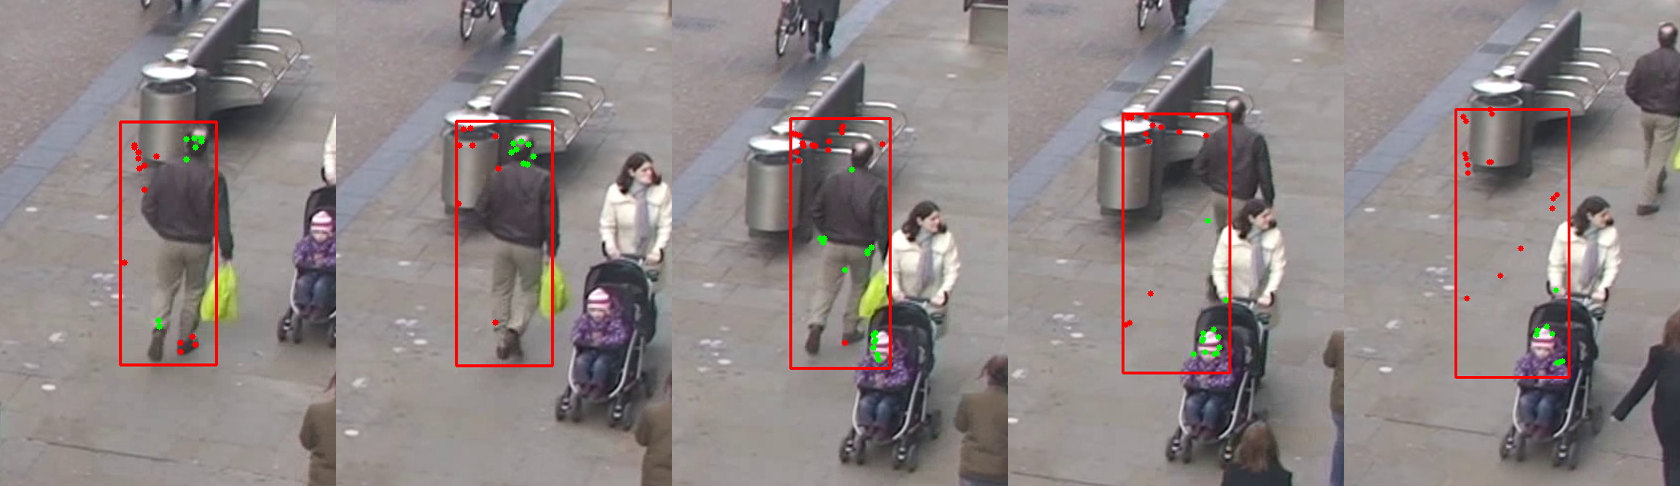
\includegraphics[width=0.9\linewidth]{velocidadas/mateuPont.png}
\caption{Tracking failure.} \label{traccs}
\end{figure}


So, we need a mechanism to detect these failures, therefore we studied how the motion algorithm behaves in these situations. When it has got a trajectory without crossing with other pedestrian, the vertical and horizontal displacement behave like a damping sine wave (if it goes away of the camera)  or amplified sine wave ( if it goes closer to the camera ). But when it has got an interference with another pedestrian, it has an steep change in that wave. We can measure that change as the differences between the current displacement and the previous one normalized by current displacement, if this value overtake a threshold, we consider that tracker as a lost track. We can observe this process in the next figure \ref{traccs23}, it belongs to previous trajectory \ref{traccs} 


\begin{figure}[H]
\centering         
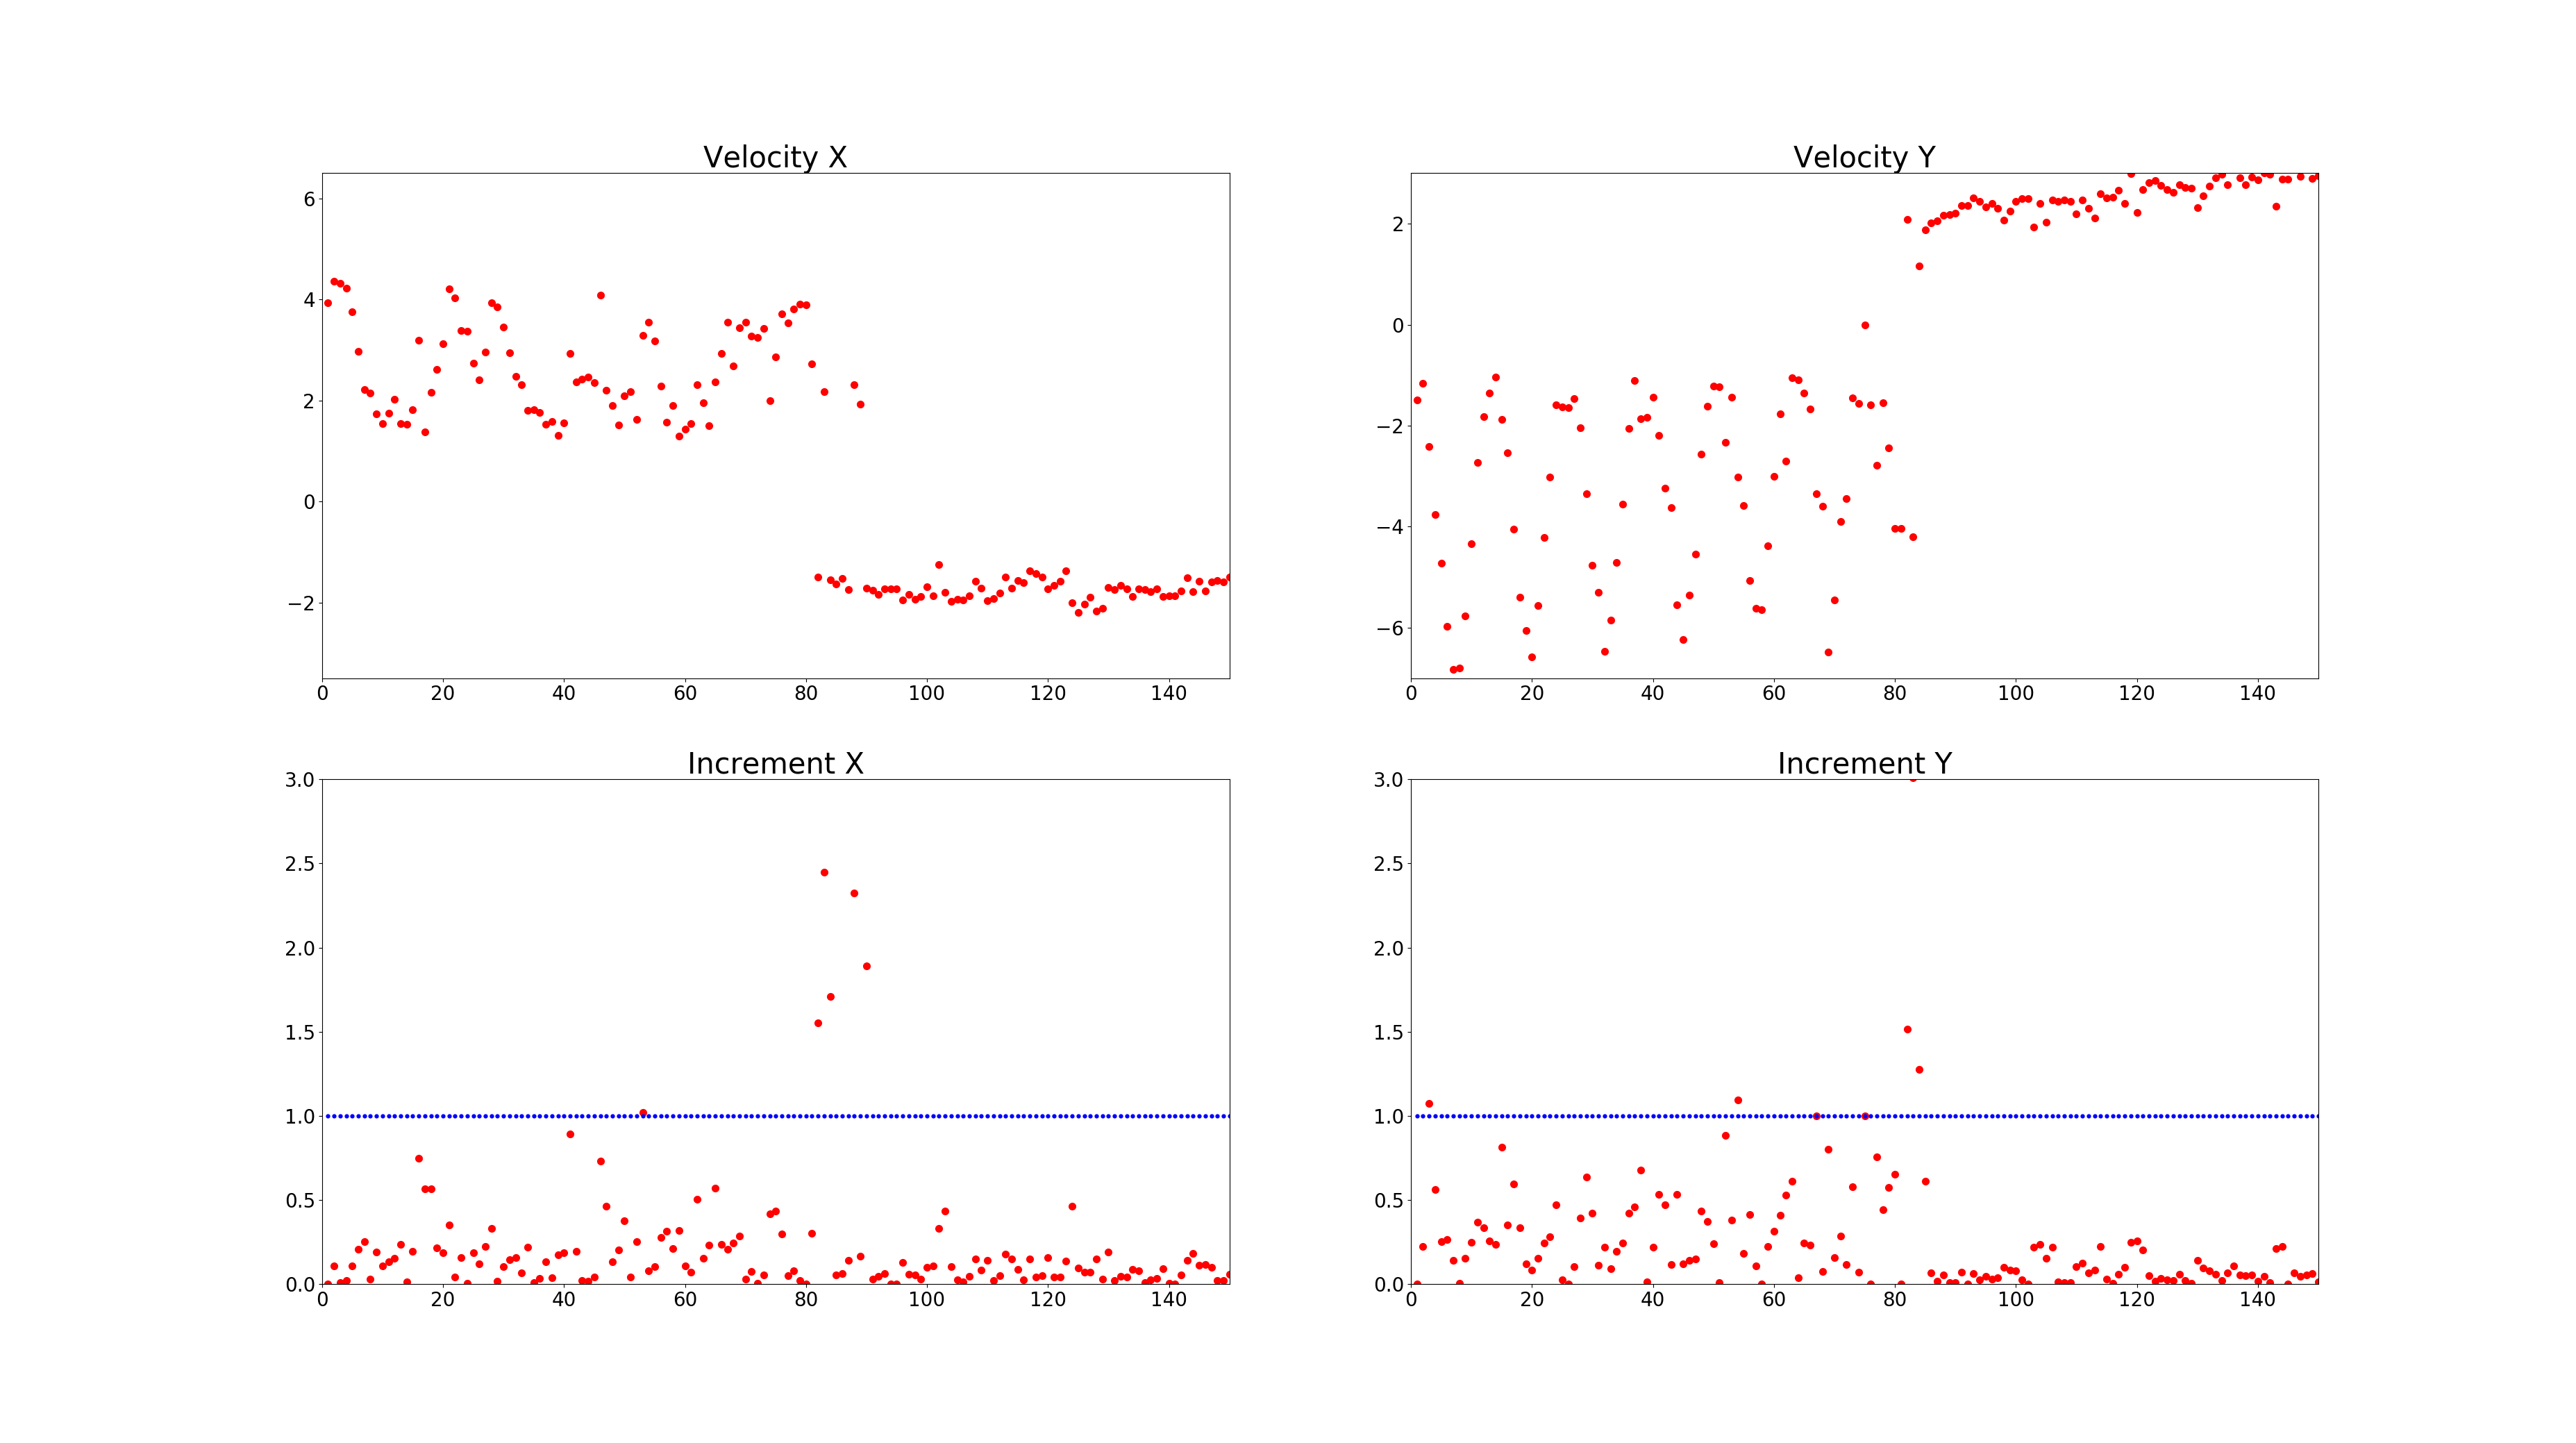
\includegraphics[width=0.9\linewidth]{velocidadas/bad_threshold.png}
\caption{Tracking failure displacements.} \label{traccs23}
\end{figure}


In contrast, when it does not cross with another pedestrian, the displacement does not get disrupt, then the normalized different with the previous displacement gets a low value, we can observe this process in figure \ref{motion2nocoorrect}. We set a threshold to notice this interference and delete this bounding box. We delete them from the current tracking execution, but we save the bounding box for following processings.

\begin{figure}[H]
		
\centering

\subfigure[Trajectory.]{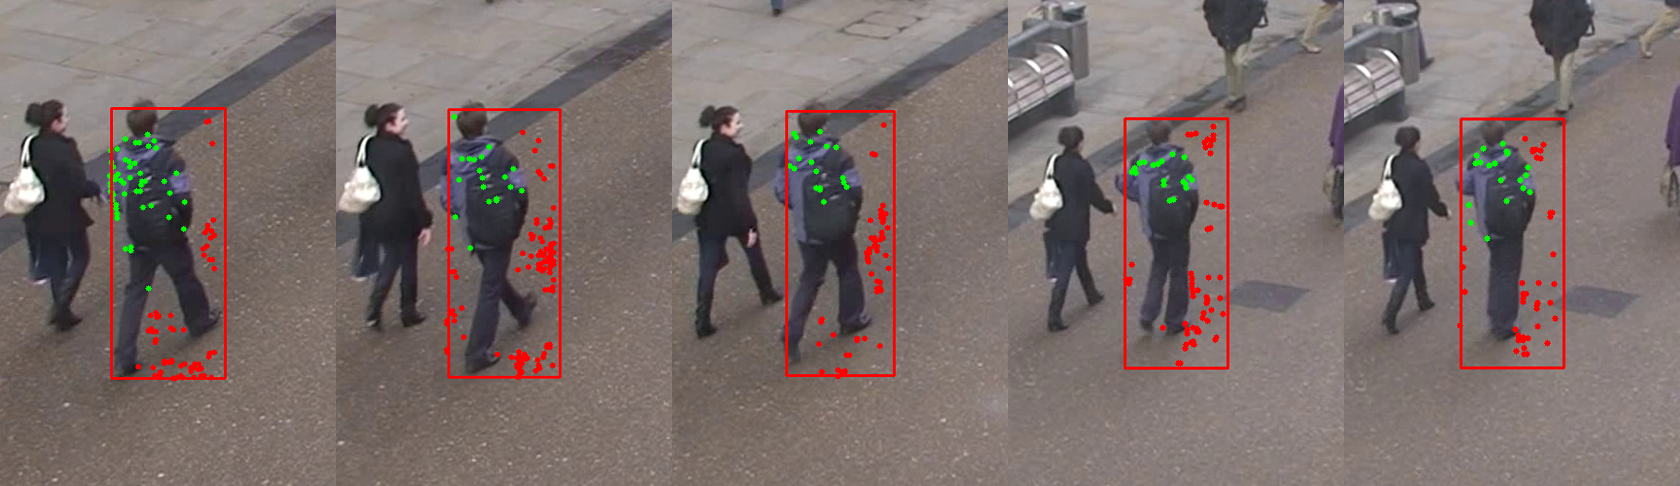
\includegraphics[width=15cm]{velocidadas/tomeuPont.png}}\\
\subfigure[Plots movement.]{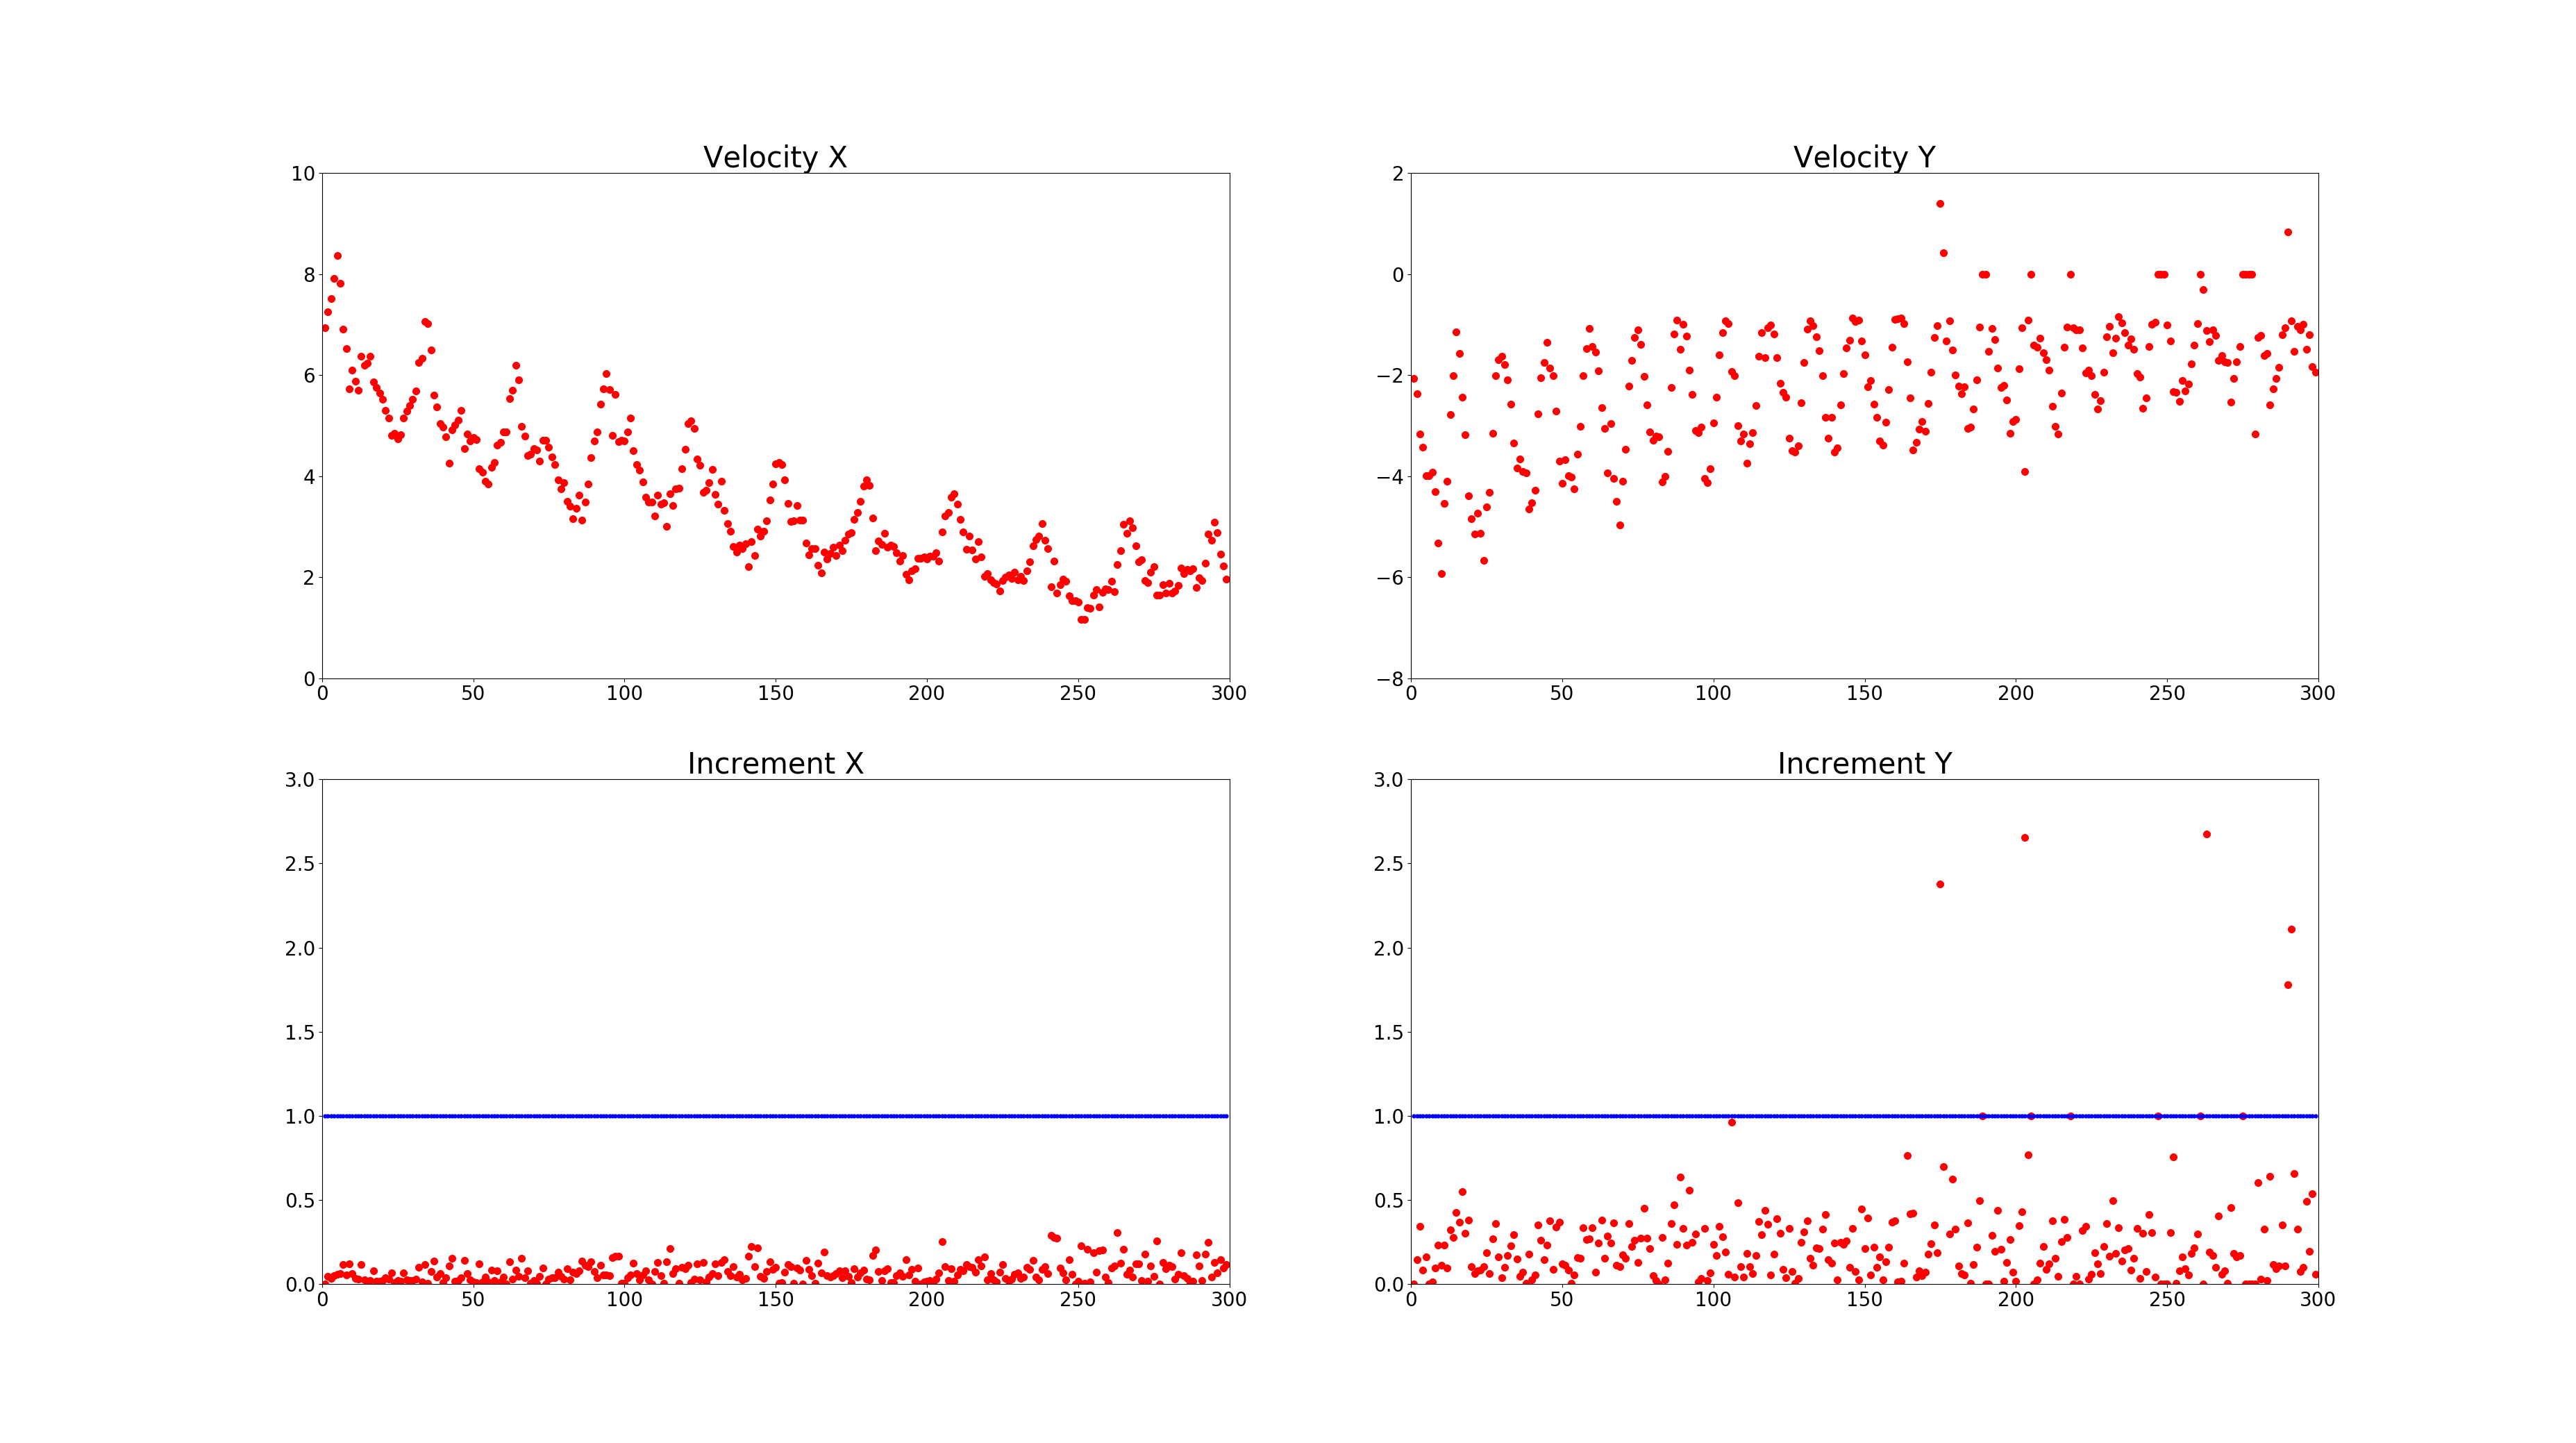
\includegraphics[width=16cm]{velocidadas/good_treshold.png}}\\
\caption{Wrong trajectory.}
\label{motion2nocoorrect}
\end{figure}













\section{Data association with detected pedestrians by the neural net}

Once we computed the trajectories, in the next iteration we might have to add a detection, so we need a module to combine these trajectories with detections. Thus, for each pedestrian we distinguish three situations:

\begin{itemize}



\item \textbf{Situation 1}, the tracket has got a nearby detection, then the detection replaces the tracket bounding box. This is what is called spatio-temporal constraint.

\item \textbf{Situation 2}, the tracket has not got a nearby detection, then the bounding box tracket continues.

\item \textbf{Situation 3}, the pedestrian has not got a tracket but has got a detection. In this case we need to decided whether this pedestrian is new in the scene or it has been seen before ( it is a lost tracket ).

\end{itemize}

We can observe the procedure for situations number one and two in the figure \ref{data1}, in green colour we can observe the detections and in blue colour the trackets. We defined nearby as the distance between the centres of the bounding boxes, this distance has to be lower than a threshold to be considered nearby. 

\begin{figure}[hptb]
\centering         
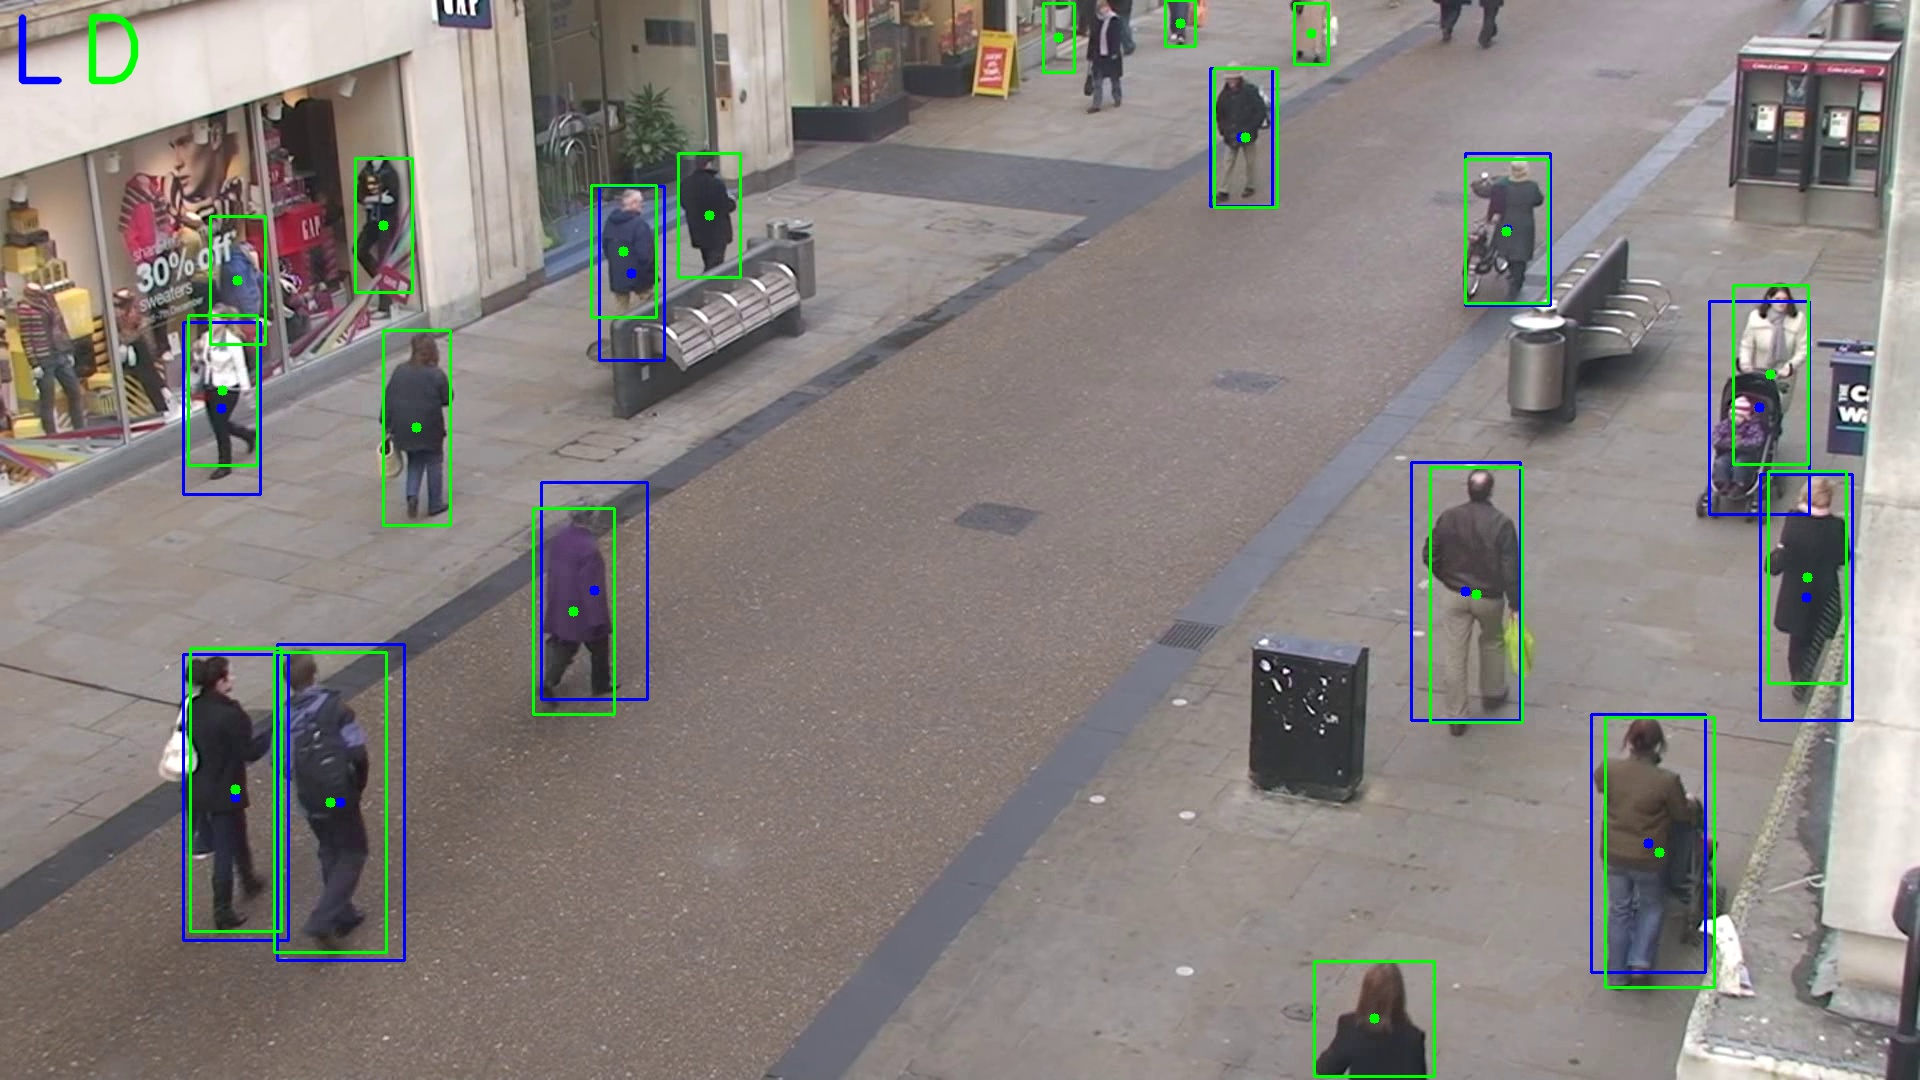
\includegraphics[width=12cm]{lucasKanade/dataAssociation.jpg}
\caption{Spatio-temporal data association.} \label{data1}
\end{figure}


To maintain the identity of the pedestrian we need a method to compare miss trackets with no associated detections, this is Situation 3. So, we decided to solve it with deep learning techniques. In particular, a Siamese convolutional neural network, with In-network architecture in \ref{saimss} we can observe a diagram and the feature dimension of each layer. This networks concatenates two blobs and computes a probability to belong to the same identity. It has got 7 convolutional layer and 1 fully connected layer, it was implemented on Keras with a Theano backend. In section \ref{exper:entrenar} we explain why we selected this architecture and how we trained it.



\begin{figure}[!]
\centering         
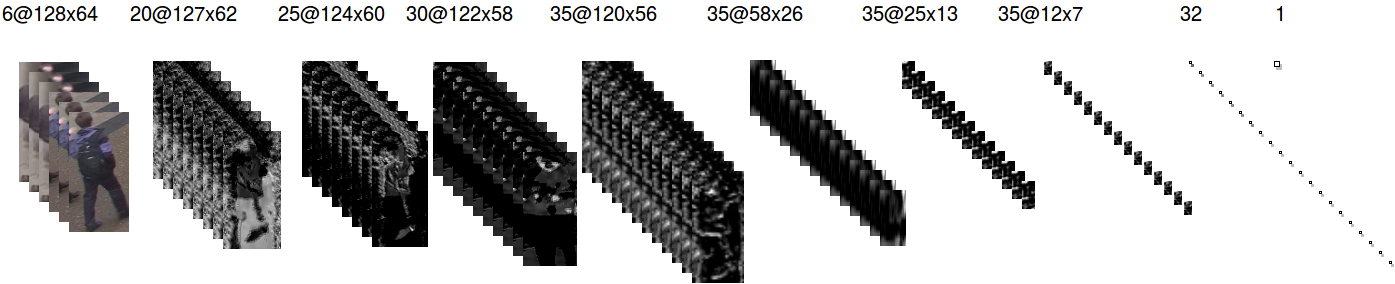
\includegraphics[width=16cm]{timesDiagram/network.png}
\caption{Siamese network: In-network.} \label{saimss}
\end{figure}


For each detection we compare with all the miss trackets, if the maximum value of this  comparision is greater than a threshold we assign it to that identity, if it is not we consider that detection as a new identity. We can observe this data association process in \ref{dataAssoc22}.



\begin{algorithm}
\caption{Data Association}\label{dataAssoc22}
\begin{algorithmic}[1]
\State \textbf{Input:} listBlobs,listDetections,listLostBlobs 
\State \textbf{Output:} listBlobs
\Procedure{Run}{}
\State $siamese = siamese.init()$
\For {$i$ in $listBlobs$}
\State $distance = euclideanDistance(blob[i],listDetections)$
\State $distanceOrdered = argmin(distance)$
\State $\%$ Situation1
\If{distanceOrdered[0] $<$ threshold}
\State newBlobs.append(listDetections[idx])
\State delete(listDetections[idx])
\State $\%$ Situation2
\Else
\State newBlobs.append(listBlobs[i])
\EndIf
\EndFor
\State $\%$ Situation3
\For {$i$ in $listDetectionsNotAssigned$}
\State $similarity = siamese.forward(listLostBlobs,DetectionsNotAssigned[i])$
\State $similarityOrdered = argmin(similarity)$
\If{similarityOrdered[0] $<$ threshold}
\State newBlobs.append(listDetectionsNotAssigned[i])
\State delete(listDetectionsNotAssigned[i])
\Else
\State newBlobs.append(listDetectionsNotAssigned[i])
\EndIf
\EndFor
\EndProcedure
\State listBlobs=newBlobs
\end{algorithmic}
\end{algorithm}


